\documentclass[aspectratio=169]{beamer}



\newcommand{\backupbegin}{
   \newcounter{finalframe}
   \setcounter{finalframe}{\value{framenumber}}
}
\newcommand{\backupend}{
   \setcounter{framenumber}{\value{finalframe}}
}

\usepackage{tikz}
\usepackage[final]{pdfpages}
\usepackage{pgffor}

\setbeamertemplate{navigation symbols}{}
\setbeamercolor{frametitle}{fg=red}
\setbeamercolor{title}{fg=white}
\setbeamercolor{author}{fg=white}
\setbeamercolor{date}{fg=white}
\setbeamerfont{frametitle}{family=\rmfamily,shape=\itshape,size=\huge} 
\setbeamerfont{title}{family=\rmfamily,shape=\itshape,size=\huge} 
\usetheme{boxes}
\setbeamertemplate{footline}[frame number]
\setbeamertemplate{itemize/enumerate body begin}{\small}
\setbeamertemplate{itemize/enumerate subbody begin}{\footnotesize}


\newcommand{\lyaf}{Lyman-$\alpha$ forest\ }
\newcommand{\lya}{Lyman-$\alpha$\ }
\newcommand{\djc}{{\color{red} !!Jaffe!!}}
\newcommand{\fix}{{\color{red} !!Fix!!}}
\newcommand{\red}[1]{{\color{red}#1}}
\definecolor{orange}{RGB}{255,127,0}
\newcommand{\orange}[1]{{\color{orange}#1}}
\newcommand{\brown}[1]{{\color{brown}#1}}
\newcommand{\blue}[1]{{\color{blue}#1}}

%
%Global Background must be put in preamble
%-rescale the 16:9 image to slide size choice
\usebackgroundtemplate{
\includegraphics[width=\paperwidth,height=\paperheight]{bnl_interior}}
%
\title{Preparation for Physics with LSST}
\author{Erin Sheldon}
\date{July 25, 2018}

\begin{document}
{\usebackgroundtemplate{
\includegraphics[width=\paperwidth,height=\paperheight]{bnl_title}}
\maketitle
}



\begin{frame}
  \frametitle{Overview of LSST  at BNL}

  \begin{center}
    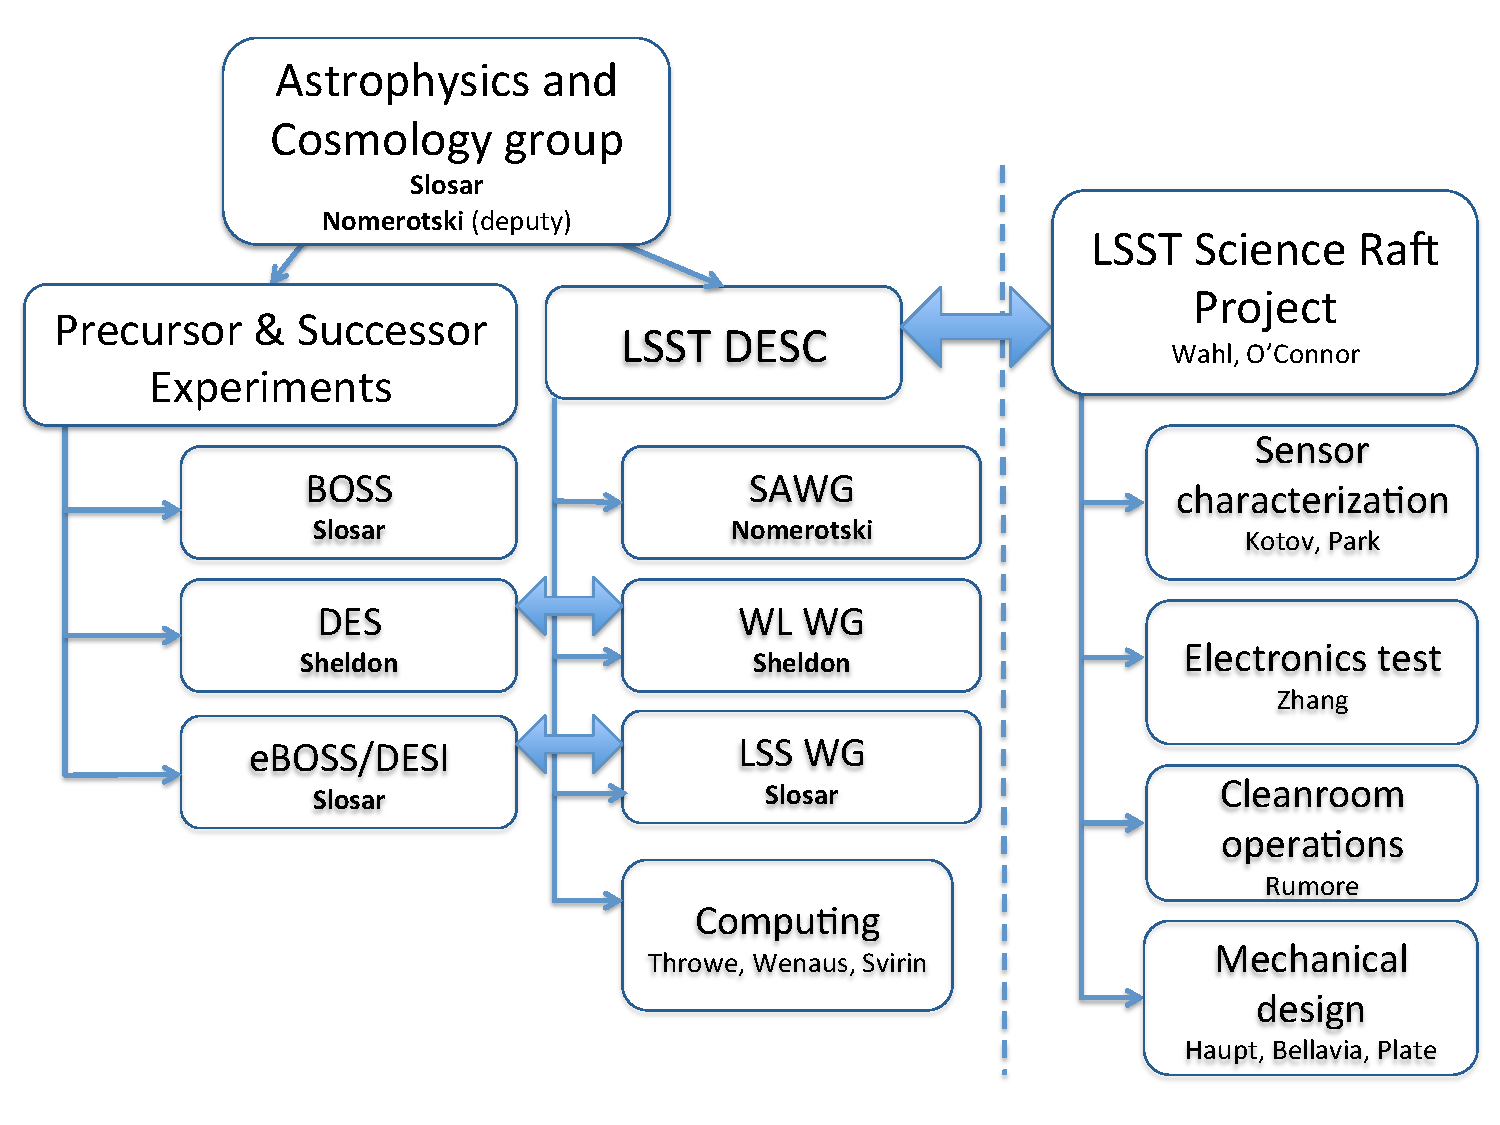
\includegraphics[height=0.8\textheight]{chart.pdf}
  \end{center}
\end{frame}

% including full pdf page
{
    \usebackgroundtemplate{%
        \parbox[c][\paperheight][c]{\paperwidth}{\centering\includegraphics[height=\paperheight]{photos.pdf}}
        }
\frame
{
}
}



% \begin{frame}

%   \frametitle{LSST project at BNL}

%   \begin{columns}
%       \begin{column}{10cm}
%           In Instrumentation Division, focus on \emph{raft production}:
%           \begin{itemize}

%               \item BNL deliverable: tower raft modules containing focal plane
%                   sensors and driver / readout electronics

%               \item BNL deliverable is performance and schedule critical

%               \item Production in full swing but ramping down 

%               \item There is approximately \$1.5 mil of LSST project funding to  flow
%                   through IO by $\sim$ 3/19 (down from peak $\sim$\$5mil)

%               \item LSST (Science Raft) has approximately 8 full time employees and the
%                   equivalent of about 2 FTEs of contract labor support 

%               \item Science Raft Subsystem Manager and Subsystem Scientist are BNL
%                   employees at IO

%               \item See full talks by Nomerotski and O'Connor

%           \end{itemize}
%       \end{column}
%       \begin{column}{5cm}
%           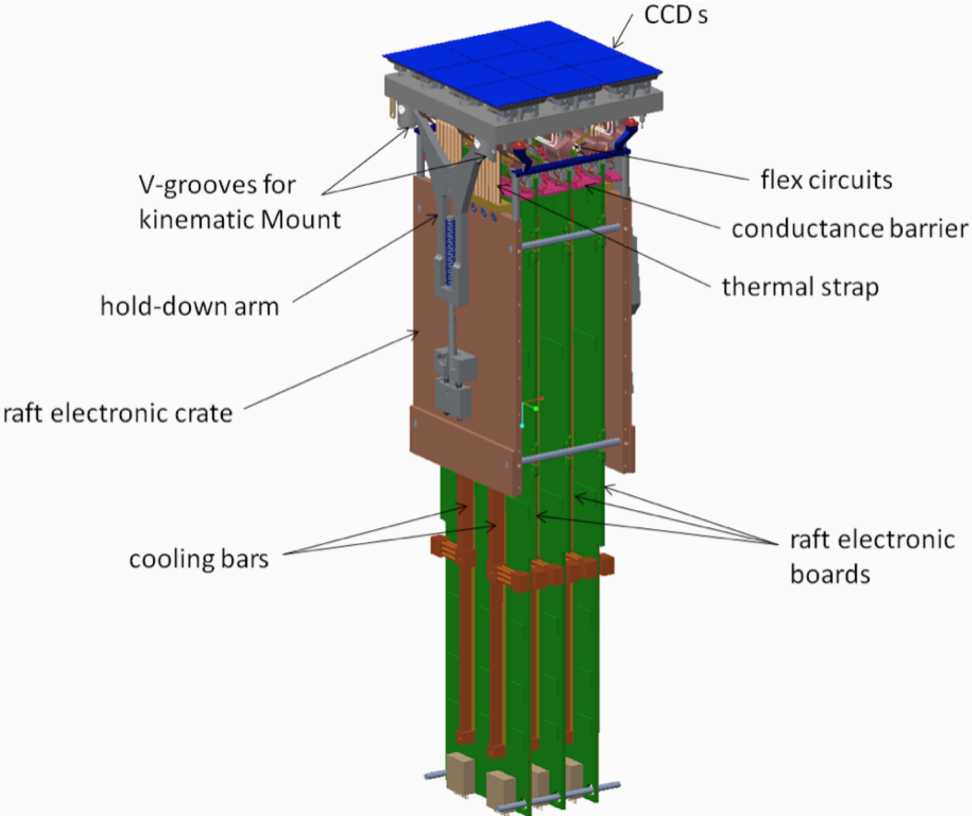
\includegraphics[width=\linewidth]{./lsstraftx.png}
%       \end{column}
%   \end{columns}


% \end{frame}



\begin{frame}

  \frametitle{BNL role in LSST camera}

  \begin{columns}
      \begin{column}{10cm}

          \begin{itemize}

          \item Instrumentation Division has been involved in the
            design and development of the focal plane modules for the
            last 15 years 

          \item BNL deliverables: 

            \begin{itemize}
            \item tower raft modules containing focal plane sensors
              and driver / readout electronics 
            \item commissioning camera, cryostat and test-raft
            \end{itemize}

              \item Raft production is in full swing but ramping down,
                scheduled to complete in Q2 FY19

              \item Science Raft Subsystem Manager and Subsystem Scientist are BNL
                  employees at IO

              \item See full talks by Nomerotski and O'Connor

          \end{itemize}
      \end{column}
      \begin{column}{5cm}
          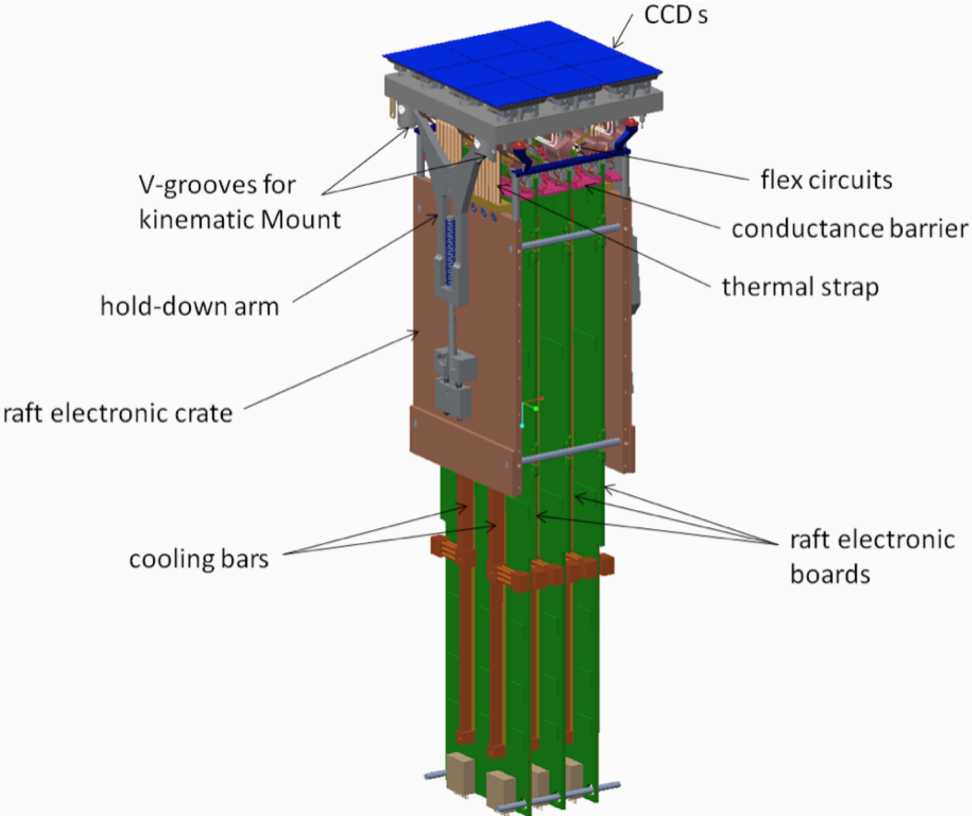
\includegraphics[width=\linewidth]{./lsstraftx.png}
      \end{column}
  \end{columns}


\end{frame}



\begin{frame}
    \frametitle{Dark Energy Science Collaboration (DESC) Leadership roles}

    \begin{itemize}

        \item \textbf{Tom McClintock}
            \begin{itemize}
                \item Joining BNL as a postdoc in the fall
                \item Leading cosmology with galaxy
                    clusters using Data Challenge 2 (DC2)
            \end{itemize}

        \item \textbf{Andrei Nomerotski}:
            \begin{itemize}
                \item co-convenor of Sensor Anomalies Working Group
                \item Chair of the DESC Membership committee
                \item member of Collaboration Council
            \end{itemize}


        \item \textbf{Erin Sheldon}:
            \begin{itemize}
                \item WL pipeline Scientist (technical lead)
                    %\item partly supported on DESC  operations funding
                \item WL shear group convenor in DES (LSST precursor)
            \end{itemize}

        \item \textbf{An\v{z}e Slosar}: 
            \begin{itemize}
                \item co-convenor of Large Scale Structure Working Group
                \item member of the LSST Science Advisory Committee (LSST project role)
                \item former member of Collaboration Council, Meetings Committee
                \item helped draft the \emph {DESC Code of Conduct}

            \end{itemize}

    \end{itemize}

\end{frame}

\begin{frame}
  \frametitle{LSST University Connections}

  \begin{itemize}


    \item \textbf{Stony Brook}:
        \begin{itemize}
      \item Three cosmology faculty at Stony Brook: Neelima Sehgal
        (recently tenured), Anja von der Linden (DOE EC for clusters),
        Marilena Loverde (DOE EC for neutrino large scale structure).
        
      \item Dmitri Tsybyshev co-supervises HyeYun Park, SB grad
        student working in LSST cleanroom and data analysis
        \end{itemize}


    \item \textbf{Harvard:}
        \begin{itemize}
            \item Regularly work with Stubbs' group on instrumentation
                issues
            \item Collaborated on monocam (see AN talk)
        \end{itemize}

    \item \textbf{Princeton:}
        \begin{itemize}
            \item Strong connections on data reduction and management.  Sheldon
                \& Bob Armstrong developing new image coaddition code.
            \item Former BNL postdoc Fisher-Levine moved to Princeton to
                work on LSST data management
        \end{itemize}
    \item \textbf{Oxford:}
        \begin{itemize}
          \item postdoc Dan Weatherill collaborating on sensor
            anomalies work
          \item regular visits and exchanges
          \item David Alonso: co-convener of LSS WG, papers and
            analysis tools
        \end{itemize}

\end{itemize}
\end{frame}


\begin{frame}
  \frametitle{LSST University Connections}

  \begin{itemize}

    \item \textbf{University of Pennsylvania }:
        \begin{itemize}
            \item Sheldon and Jarvis (U. Penn) co-convene the DES Weak Lensing 
                shear pipeline working group and collaborate closely on WL science
        \end{itemize}


    \item \textbf{Wayne State University}:
      \begin{itemize}
          \item Rebecca Coles (SCGSR student) worked in LSST cleanroom
            for two years
      \end{itemize}


    \item \textbf{University of Prague}:
      \begin{itemize}
          \item Several long term visitors with Nomerotski
          \item Work on sensor effects, software for CCD image analysis
      \end{itemize}




\end{itemize}
\end{frame}




\begin{frame}
  \frametitle{LSST DESC Collaboration Meeting 2017 }
  
  \begin{columns}
    \begin{column}{0.4\textwidth}
      \begin{itemize}
    \item BNL hosted the summer 2017 DESC meeting, organized jointly
        with Stony Brook.
      \item The choice of BNL as host is a recognition of the important role
          BNL plays in the collaboration

      \end{itemize}
    \end{column}
    \begin{column}{0.6\textwidth}
      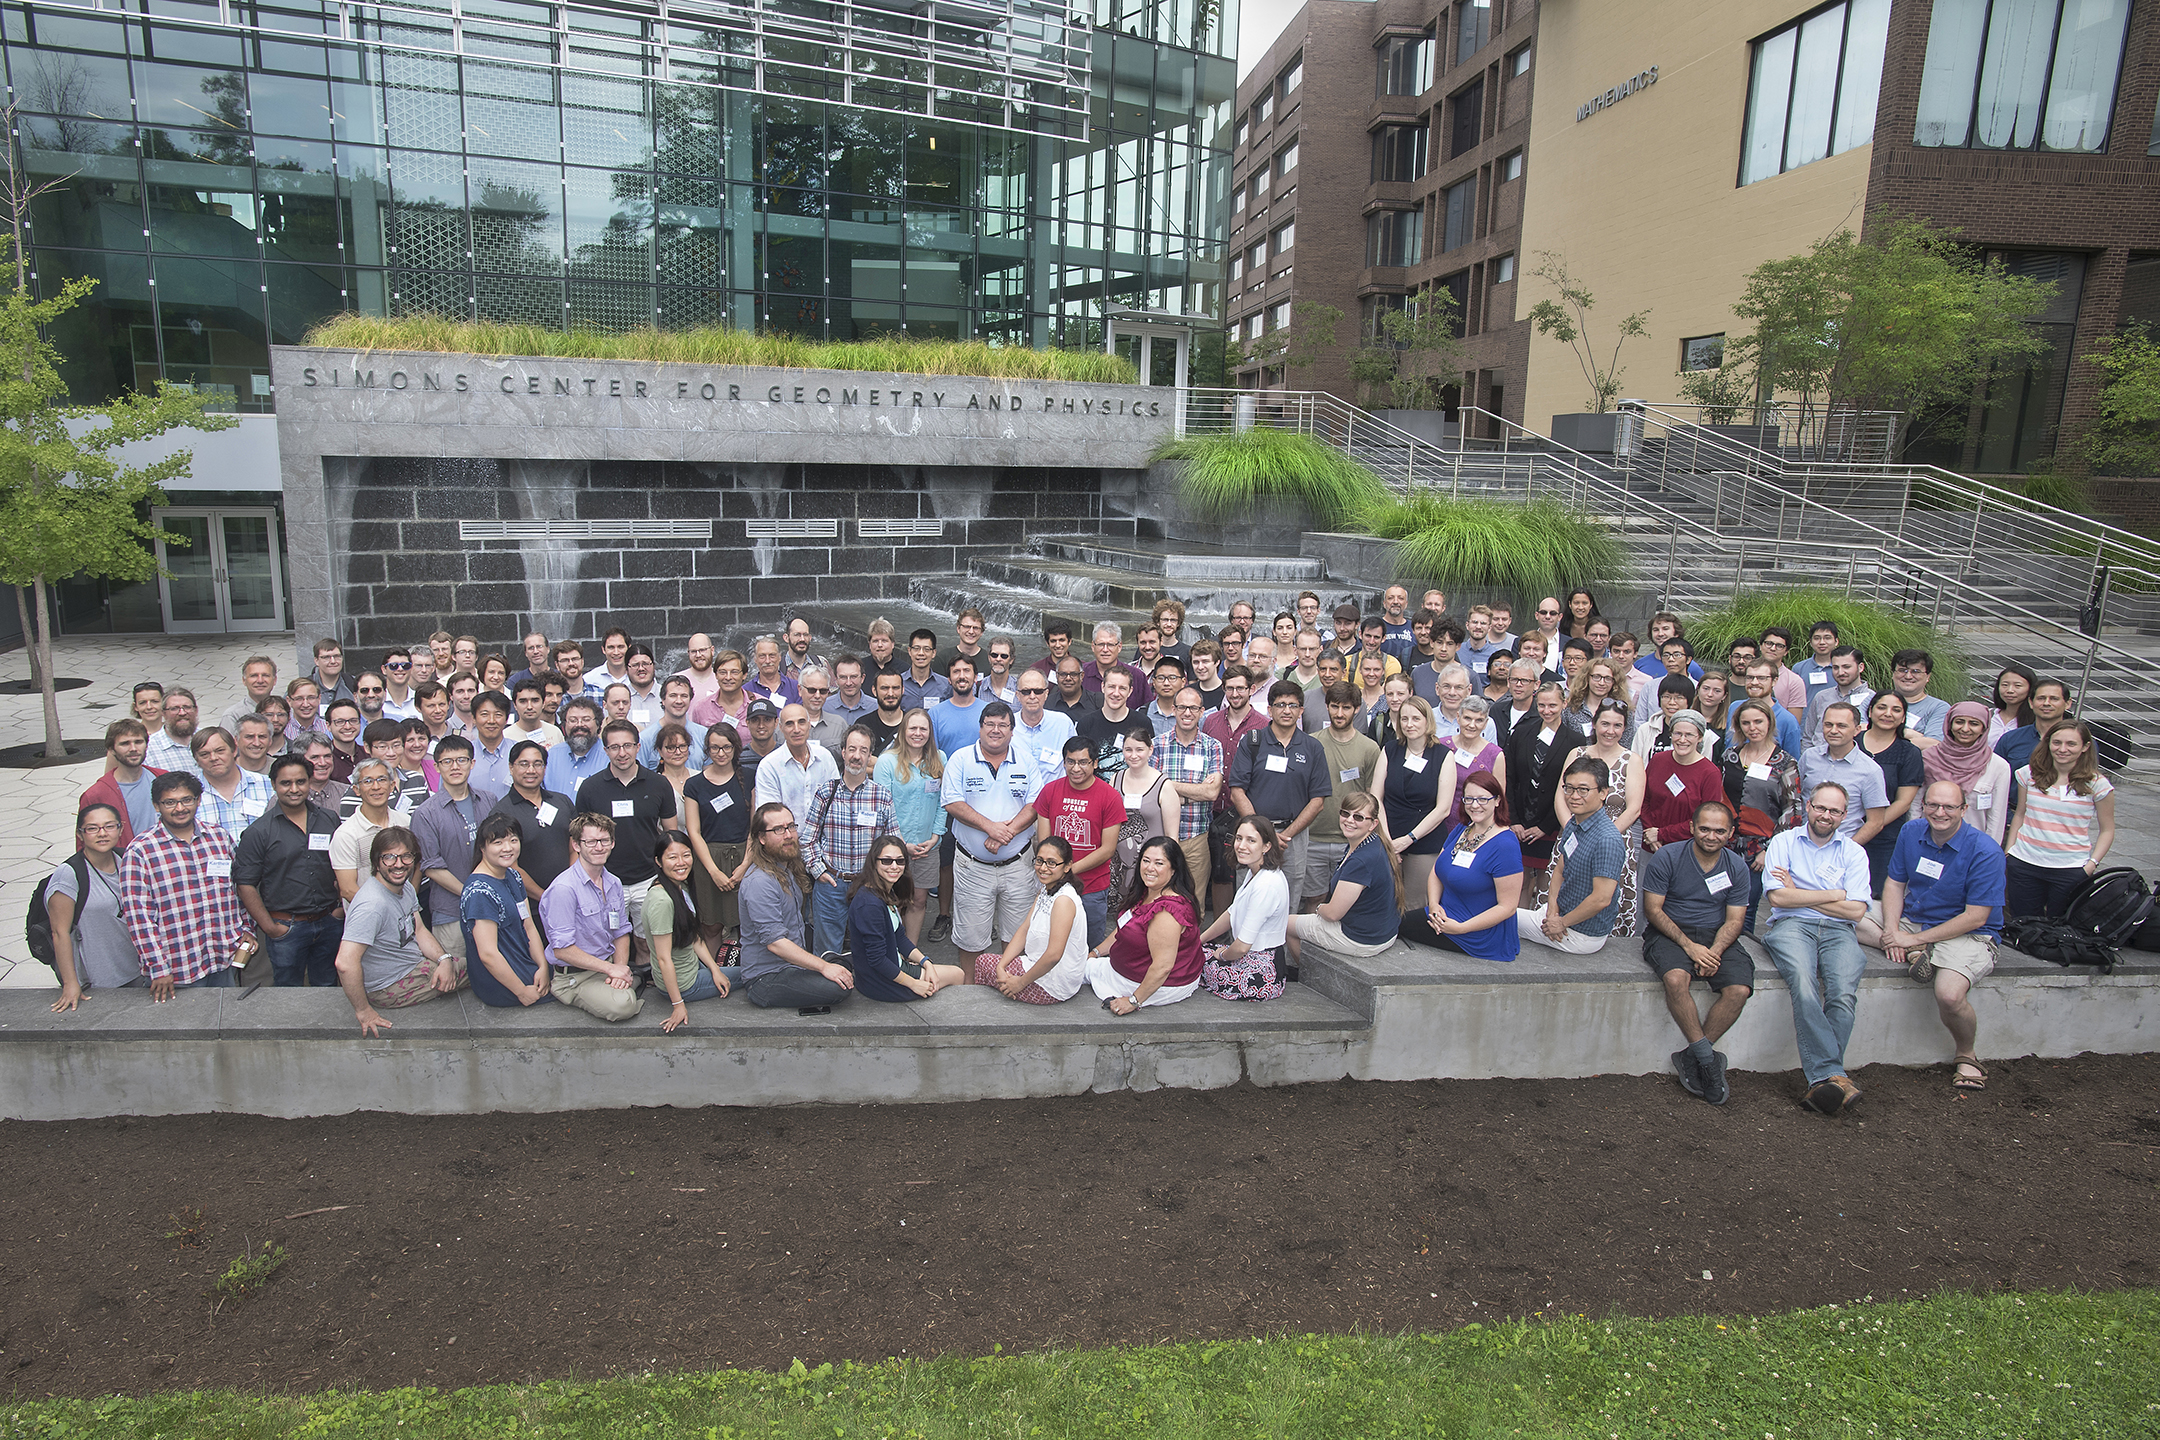
\includegraphics[width=\linewidth]{./D0680717.jpg}
    \end{column}
  \end{columns}


\end{frame}

% including full pdf page
{
    \usebackgroundtemplate{%
        \parbox[c][\paperheight][c]{\paperwidth}{\centering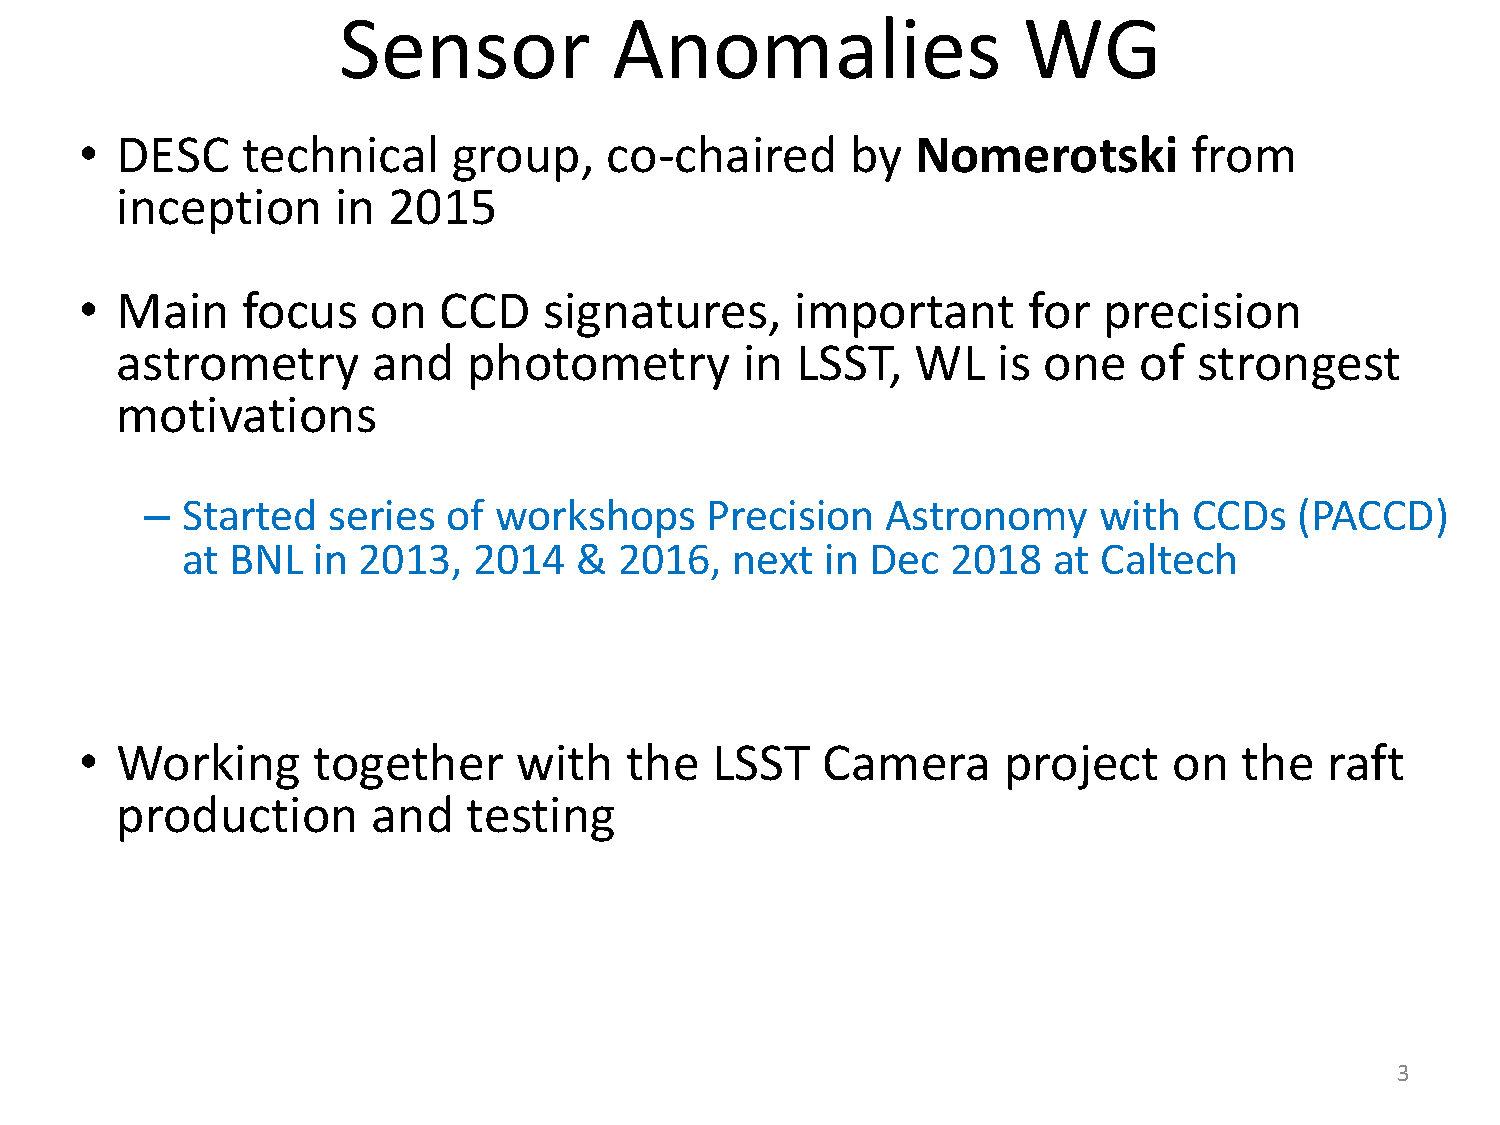
\includegraphics[height=\paperheight]{sawg.pdf}}
        }
\frame
{
}
}



\begin{frame}
\frametitle {DESC Large Scale Structure WG}

    \begin{itemize}  
        \item co-chaired by \textbf{Slosar} since January 2016 with David
            Alonso (Oxford)

        \item Actively developing the 3x2pt pipeline infrastructure and
            novel analysis tools with others in the LSS group:
            \begin{itemize}
                \item Slosar developed the \texttt{sacc} container class that will
                    hold correlations, covariance matrices, etc. for the official
                    pipeline

                \item Slosar contributed to \texttt{NaMaster}, the power
                    spectrum estimation tool with capability for full mode projects,
                    etc (main developer David Alonso, paper to be ready soon)
            \end{itemize}

        \item In addition to infrastructure: four active research projects:

            \begin{itemize}
                \item 2pt validation: full quick analysis loop for testing effect of 
                    systematics on recovered cosmological parameters

                \item HSC data re-analysis

                \item Understanding data reduction and blending through DC2
                    input-output catalog matching

                \item In conjuction with TJP, we have begun working on project to
                    understand modeling beyond linear bias for LSST (co-leading with
                    Jonathan Blazek)

            \end{itemize}


    \end{itemize}

\end{frame}


\begin{frame}
  \frametitle{2pt validation project}
  
  \begin{columns}
    \begin{column}{8cm}
      \begin{itemize}
        \scriptsize
      \item Lognormal mocks provide a quick short-cut to ``realistic
        enough'' galaxy fields
      \item These fields can be mocked using the full complexity, to
        lend more control and study systematic effects one by one:
        \begin{itemize}
\scriptsize
        \item photo-z errors
        \item depth fluctuations
        \item stellar contamination
        \item blending
        \item \ldots
        \end{itemize}
      \item In contrast to DCx challenges, we can have O(1000) mocks,
        allowing systematic statistical testing
      \item Basic framework in place
      \end{itemize}




      \vspace*{-0.7cm}
      \hfill 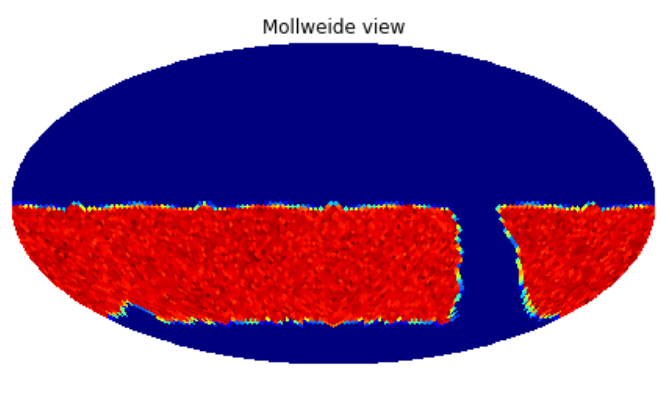
\includegraphics[width=0.50\linewidth]{./random2pt.png}

       \hfill \tiny Window function for lognormal mocks based on OpSim runs


    \end{column}
    \begin{column}{5cm}
      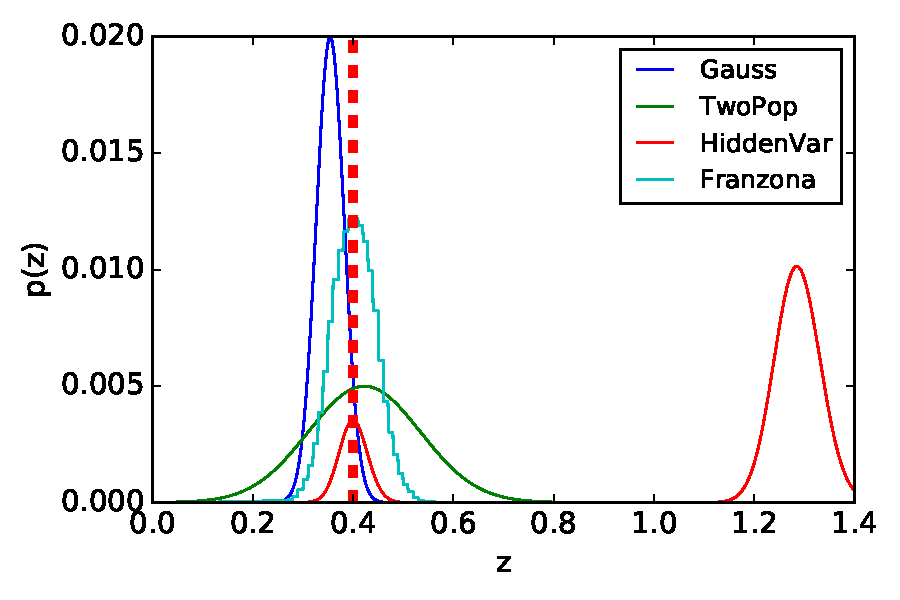
\includegraphics[width=\linewidth]{./ptest04.pdf}
      \vspace*{-0.3cm}
      \begin{center}
        \tiny Different photo-z models developed for 2-pt validation
      \end{center}

      \begin{center}
        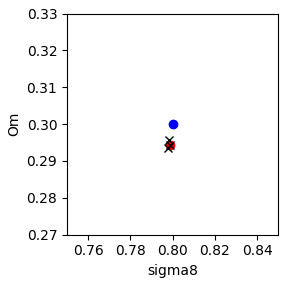
\includegraphics[width=0.6\linewidth]{./xx.png}

        \tiny First full round-trip recovering the input $\Omega_M$
        and $\sigma_8$ with small, but non-negligible biases

      \end{center}
    \end{column}
  \end{columns}
\end{frame}


\begin{frame}
  \frametitle{HSC reanalysis}

  \begin{columns}
    \begin{column}{7cm}
      \begin{itemize}
      \item Idea is to test the DESC pipeline tools on HSC data
      \item The upstream data management tools are the same for LSST
        and HSC (led by Princeton group), making it a natural testbded

      \item Tools not quite ready, but trying to use them makes all
        the deficiencies obvious
      \item Goal is to measure power-spectrum of galaxy clustering and
        characterise bias evolution of likely LSST source
      \item Stretch goal is to detect magnification
      \end{itemize}
    \end{column}
    \begin{column}{6cm}
      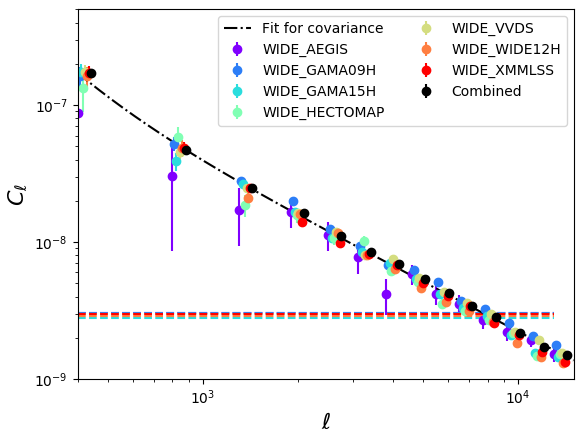
\includegraphics[width=\linewidth]{./cls_hsc_new.png}
      \begin{center}
        \scriptsize Preliminary re-analysis of HSC data. Measured
        power-spectrum consistent across fields and theoretical expectation.
      \end{center}

    \end{column}
  \end{columns}


\end{frame}


\begin{frame}
  \frametitle{DC2 matching}

  \begin{columns}
    \begin{column}{8cm}
      \begin{itemize}
        \scriptsize
      \item Connecting input and output catalogs is non-trivial
      
      \item We want to do matching with minimal assumptions and
        flagging in order to \emph{study} what various flags do

      \item Work done by Hye-Yun Park (SB) and Bhairav Valera (SULI)

      \item Using a novel Friends-of-friends based algorithm to
        preselect data into:
        \begin{itemize}
          \scriptsize
        \item  pure false positives (detections where
        there is nothing around in the input catalog)

      \item pure non-detections (input catalog objects without any
         detections in the output catalog)

      \item clear 1-1 matches (there is one input object and one
        output object and nothing else in the area)

      \item everything else (actual blends, wrongly identified blends,
        failed deblends, etc.)


        \end{itemize}
      \item Preliminary results very encouraging, numerous
        possibilities for true understanding of data reduction

      \end{itemize}
    \end{column}
    \begin{column}{3.5cm}
      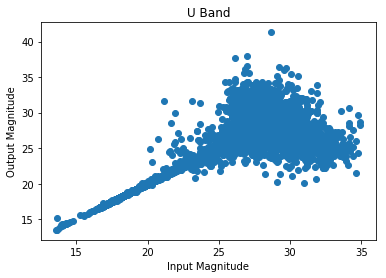
\includegraphics[width=\linewidth]{./image.png}
      \begin{center}
\scriptsize
        Input vs Output $u$-band magnitude for sources that are unique
        1-1 pairs within arcsec and are closer than 0.1 arcsec in separation
        \textit{(PRELIMINARY)}
      \end{center}
    \end{column}
    \begin{column}{3.5cm}
      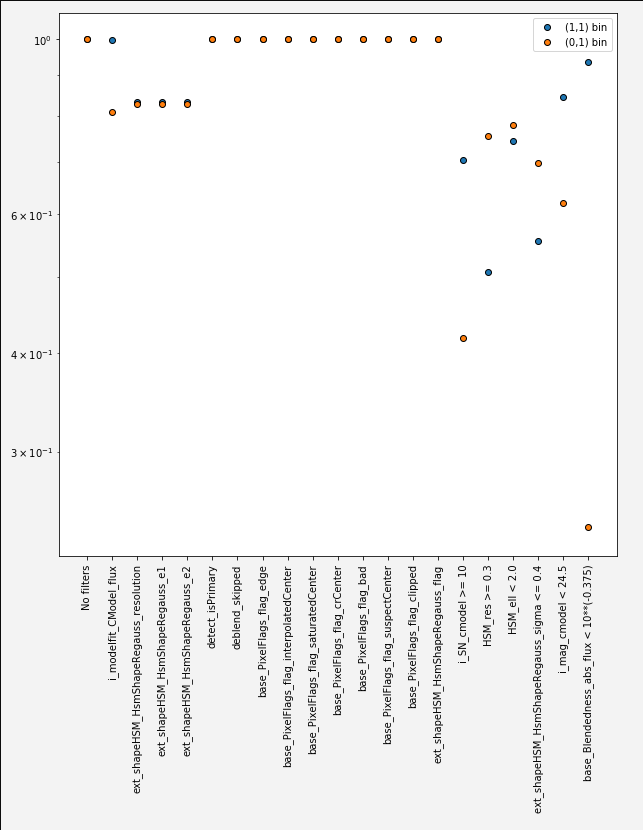
\includegraphics[width=\linewidth]{./dcmat2.png}
      \begin{center}
\scriptsize
Efficacy of HSC sample-cleaning flags on DC2 data. \textit{(PRELIMINARY)}
      \end{center}
      \end{column}



  \end{columns}



\end{frame}


\frame
{

    \frametitle{Weak Lensing Pipeline Scientist}

    \begin{columns}
        \begin{column}{0.7\textwidth}


            \begin{itemize}

                \item Erin Sheldon is a DESC 
                    pipeline scientist working on weak lensing
                    shear catalogs.

                \item Responsible for creating software 
                    pipelines to measure weak lensing shear.

                \item Responsible for producing, or coordinating
                    the production of, the shear catalogs.

                \item Adapting codes from the Dark
                    Energy Survey (metacalibration, MEDS,
                    the MOF deblender, etc.)

                \item Current focus is on reprocessing the HSC survey
                    and processing the DESC data challenge 2 (DC2)

            \end{itemize}


        \end{column}

        \begin{column}{0.3\textwidth}
            \begin{center}
                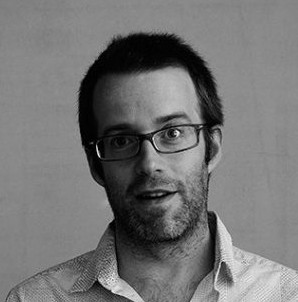
\includegraphics[width=\textwidth]{sheldon.png}
                %
\includegraphics[width=\textwidth]{TomMportrait.jpg}
                %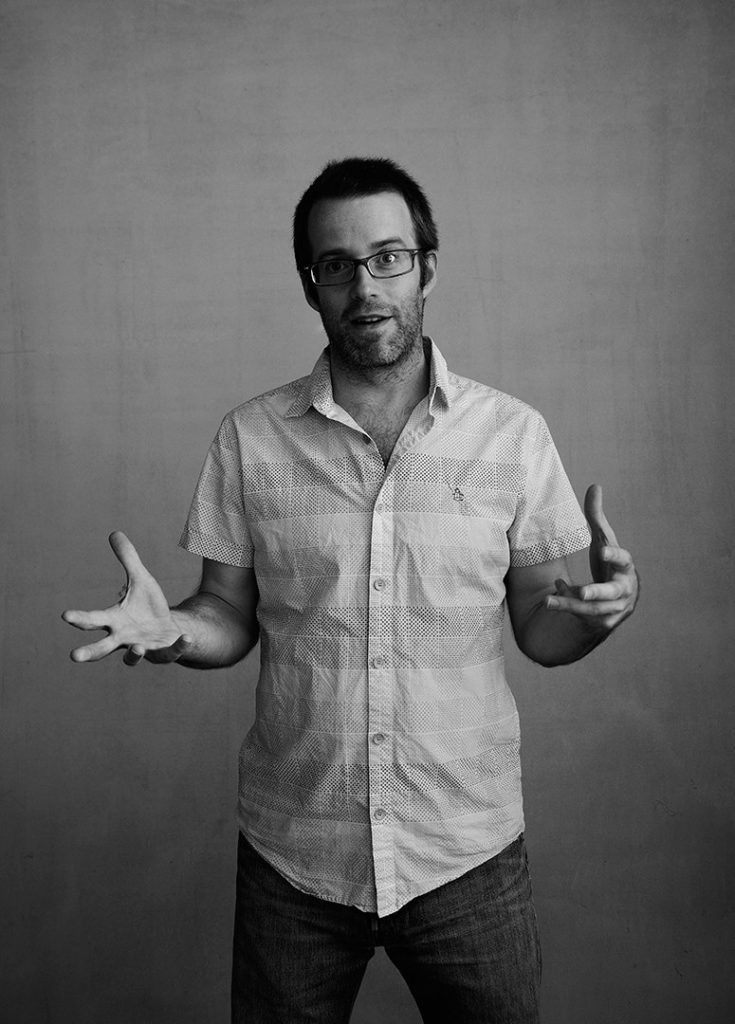
\includegraphics[width=\textwidth]{erin-sheldon-735x1024.jpg}
                \newline
                {\tiny Erin Sheldon}
            \end{center}
        \end{column}

    \end{columns}

}

% including full pdf page
{
    \usebackgroundtemplate{%
        \parbox[c][\paperheight][c]{\paperwidth}{\centering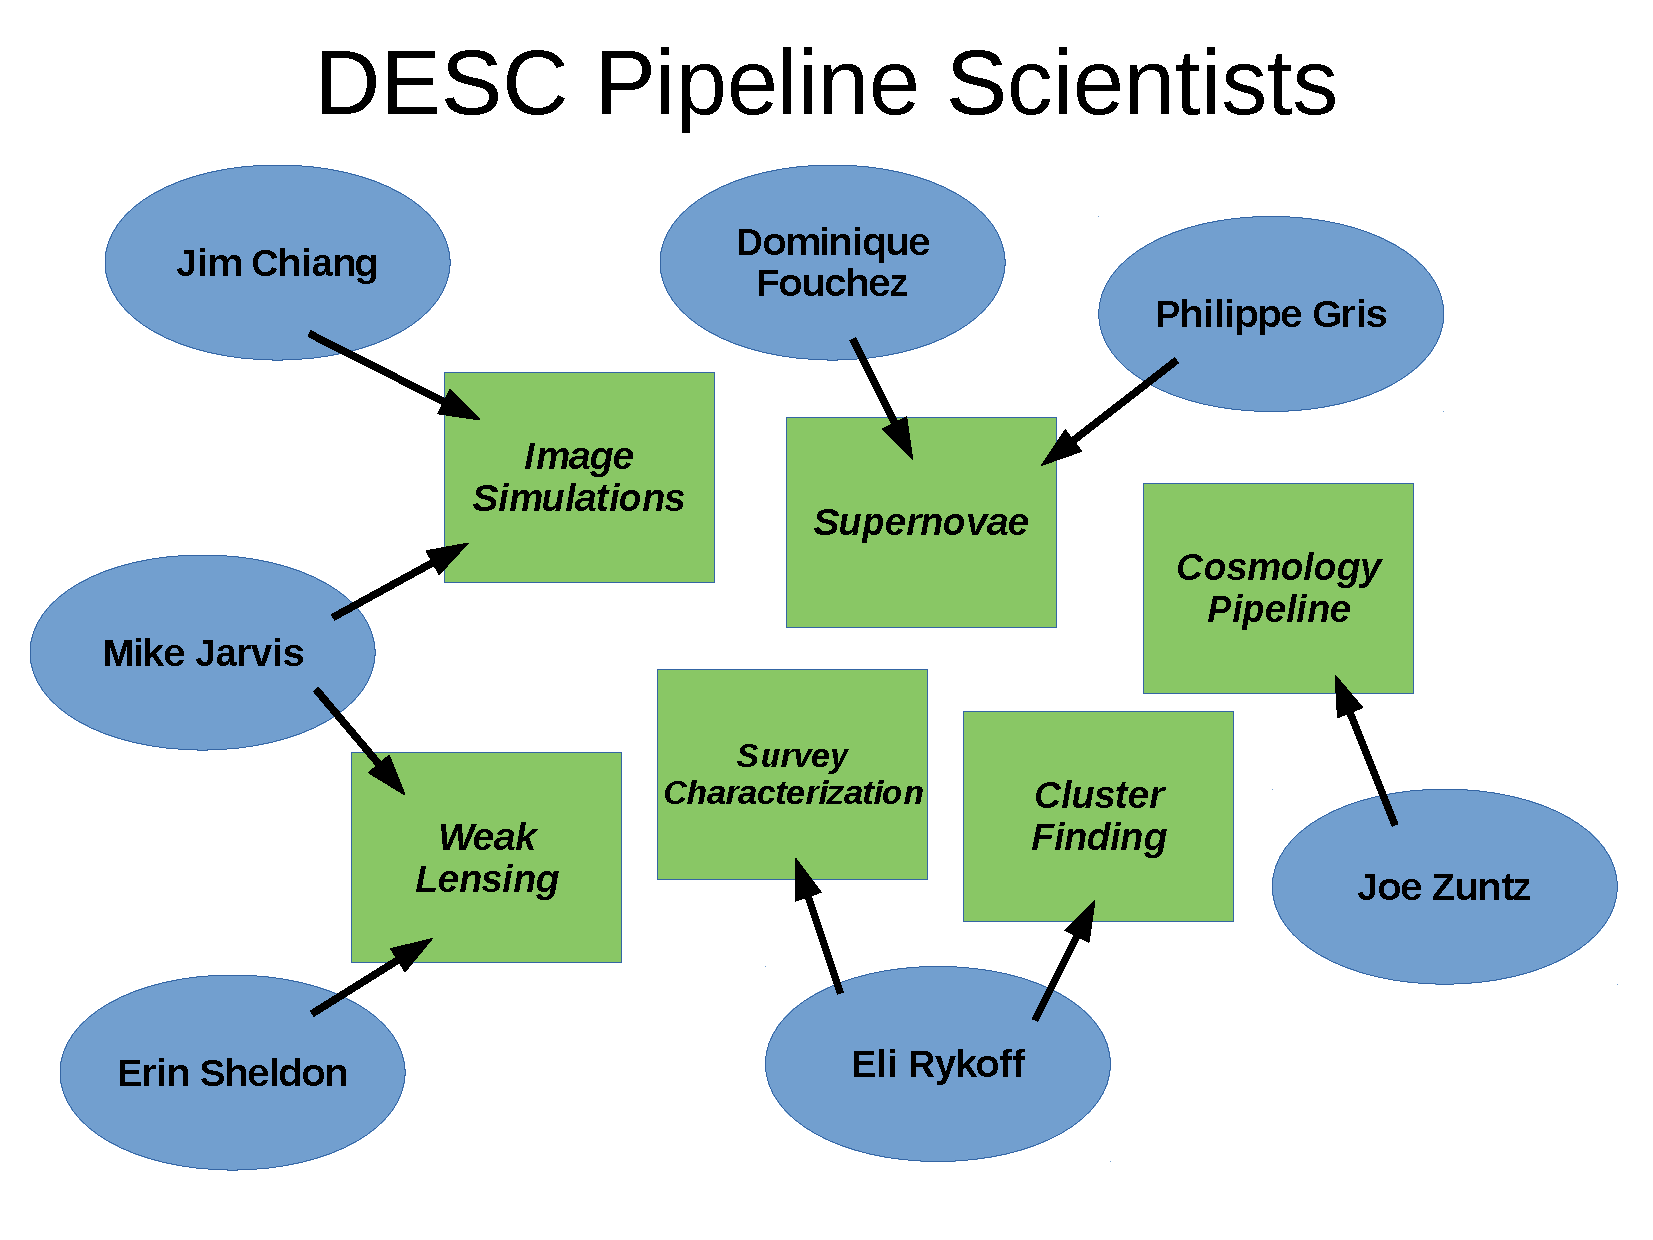
\includegraphics[height=\paperheight]{DESCPipelineScientists.pdf}}
        }
\frame
{
}
}




\frame
{

    \frametitle{Weak Lensing Pipeline Scientist: Current Progress}

    %\setbeamerfont*{itemize/enumerate body}{size=\large}

    \begin{columns}
        \begin{column}{0.5\textwidth}
            \begin{itemize}

                \item Sheldon has produced the framework to
                    use the LSST data interface (the Butler) to
                    produce the inputs needed for the shear
                    pipelines.

                \item The shear code has been run on part of the HSC data, and shear
                    catalogs produced.  Only a small subset of the data was available
                    at the time.

                \item The code is ready to run on the full HSC and DC2 when available.

            \end{itemize}
        \end{column}
        \begin{column}{0.5\textwidth}
            \centering
            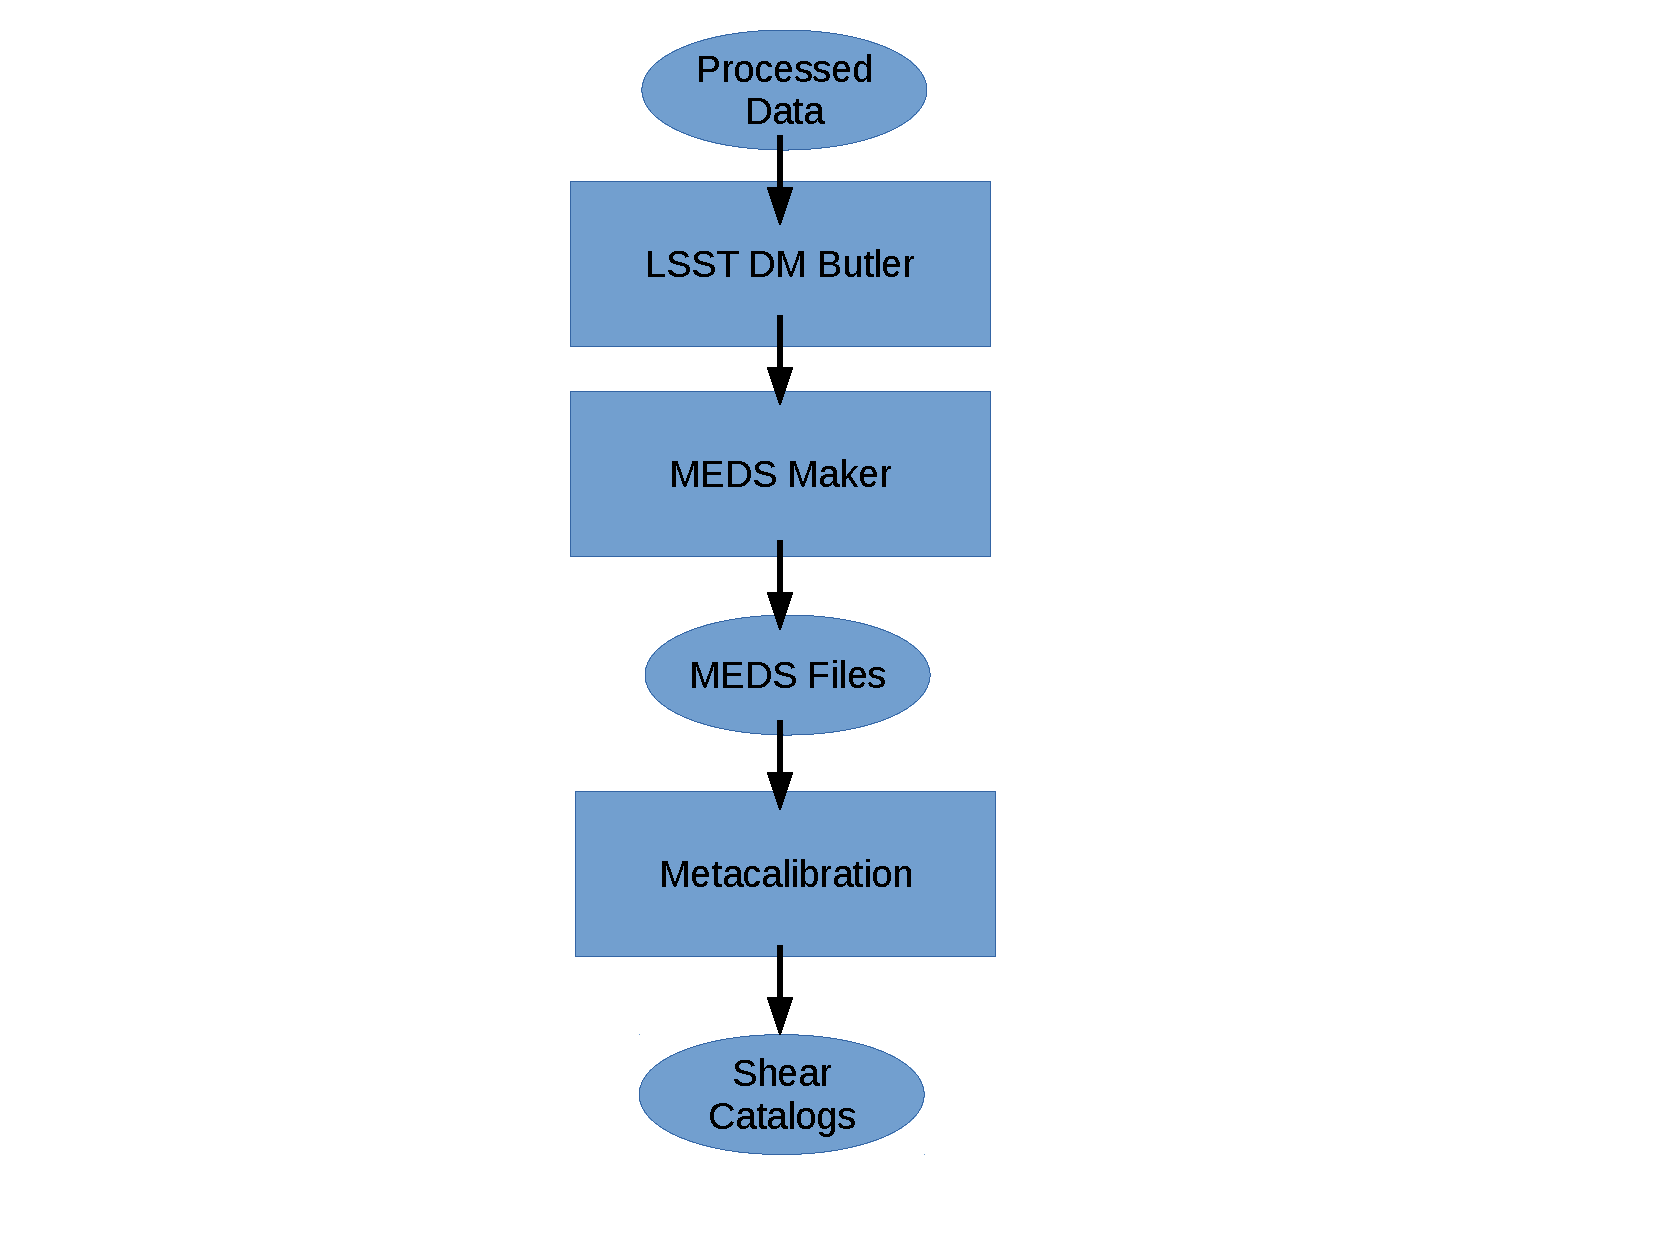
\includegraphics[width=\textwidth]{LSSTWorkflow.pdf}
        \end{column}
    \end{columns}
}

\frame
{

    \frametitle{Weak Lensing Pipeline Scientist: Immediate Future}

    %\setbeamerfont*{itemize/enumerate body}{size=\large}

    \begin{columns}
        \begin{column}{0.5\textwidth}
            \begin{itemize}

                \item Working with Francois Lanusse (CMU) to get the processing
                    of DC2 working at NERSC. Francois plans to take on the
                    actual production.

                \item Analyze the outputs

                \item Show the working group how to test and use the outputs.

                \item A new HSC reprocessing should be available soon, and
                    shear catalogs will be produced.  This could 
                    potentially lead to science papers.

            \end{itemize}

        \end{column}

        \begin{column}{0.5\textwidth}
            \centering
            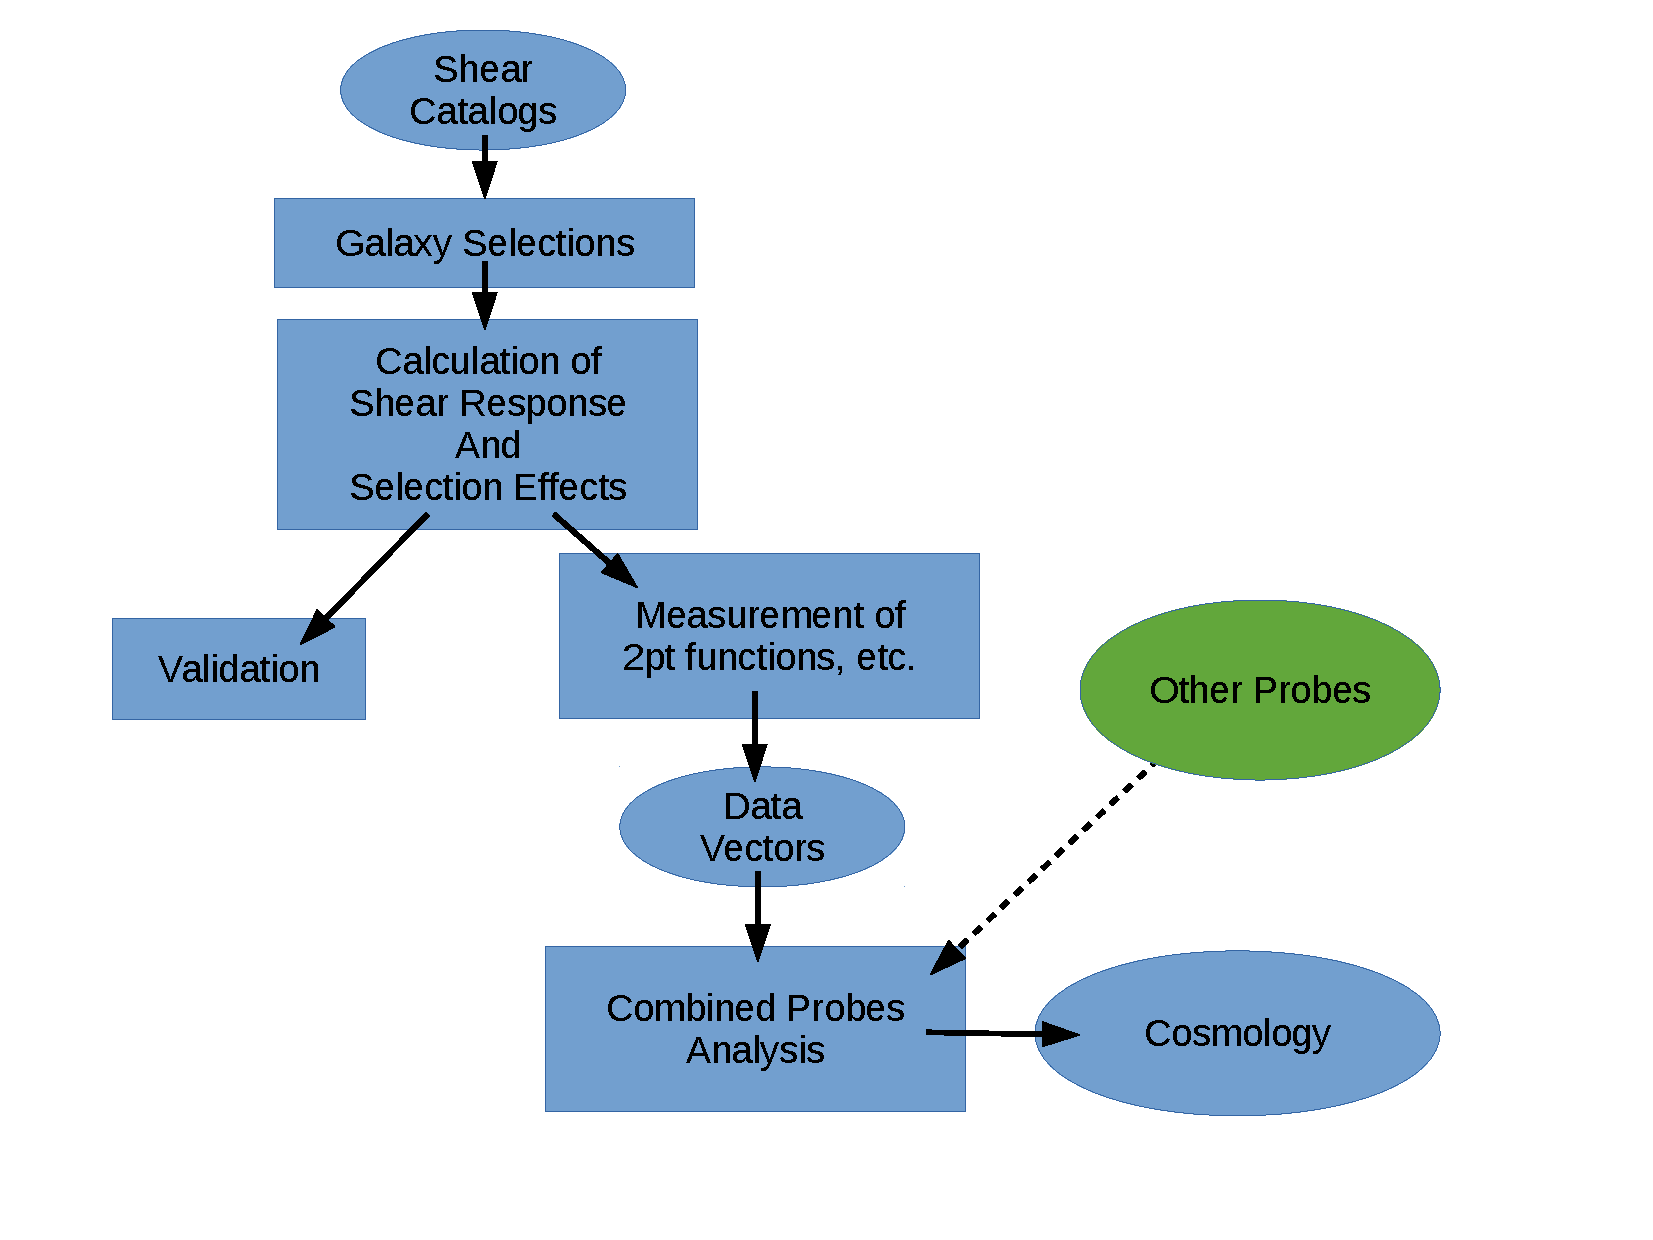
\includegraphics[width=\textwidth]{LSSTAnalysisWorkflow.pdf}
        \end{column}
    \end{columns}

}

\frame
{

    \frametitle{Weak Lensing Pipeline Scientist: Future}

    %\setbeamerfont*{itemize/enumerate body}{size=\large}

    \begin{columns}
        \begin{column}{0.5\textwidth}

            \begin{itemize}

                \item Get other DES codes working as well: MOF Image Deblender.  LSST
                    has higher object density than DES.  Currently testing this regime
                    using deep fields from DES.

                \item Help to prepare other codes, e.g. BFD (Bernstein et al.)

                \item Get some of the interface code worked into LSST DM

            \end{itemize}

        \end{column}

        \begin{column}{0.5\textwidth}
            \centering
            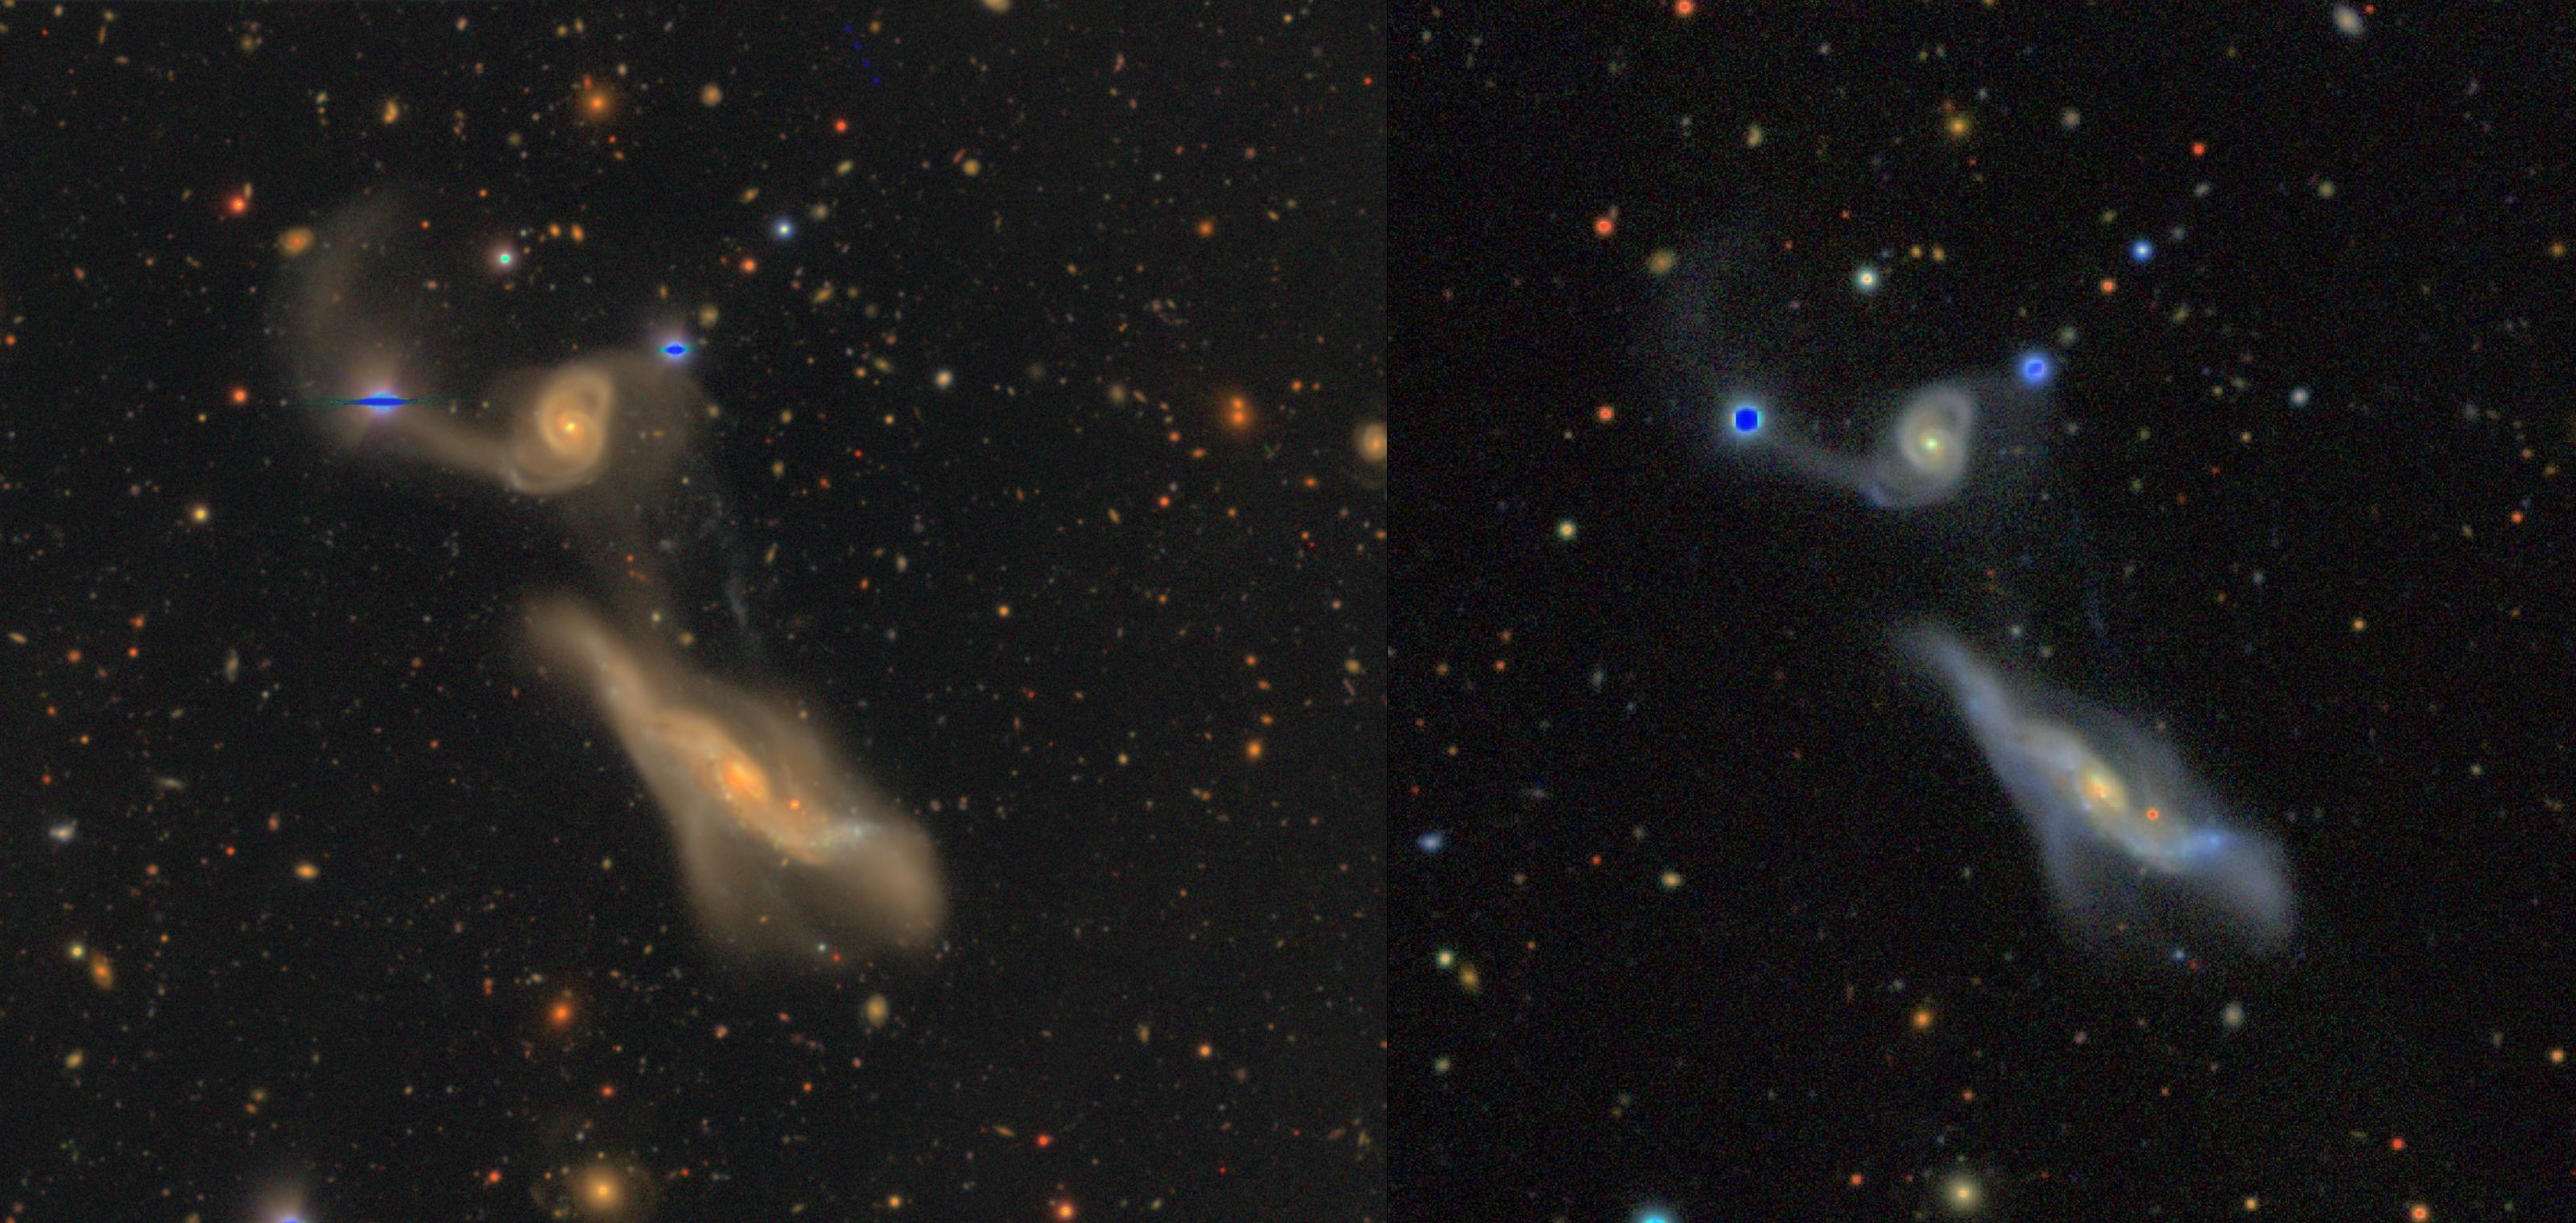
\includegraphics[angle=90,height=0.8\textheight]{HSC-DES-interacting-pair.jpg}
        \end{column}
    \end{columns}


}

{
    \usebackgroundtemplate{%
        \colorbox{black}{ \parbox[c][\paperheight][c]{\paperwidth}{\centering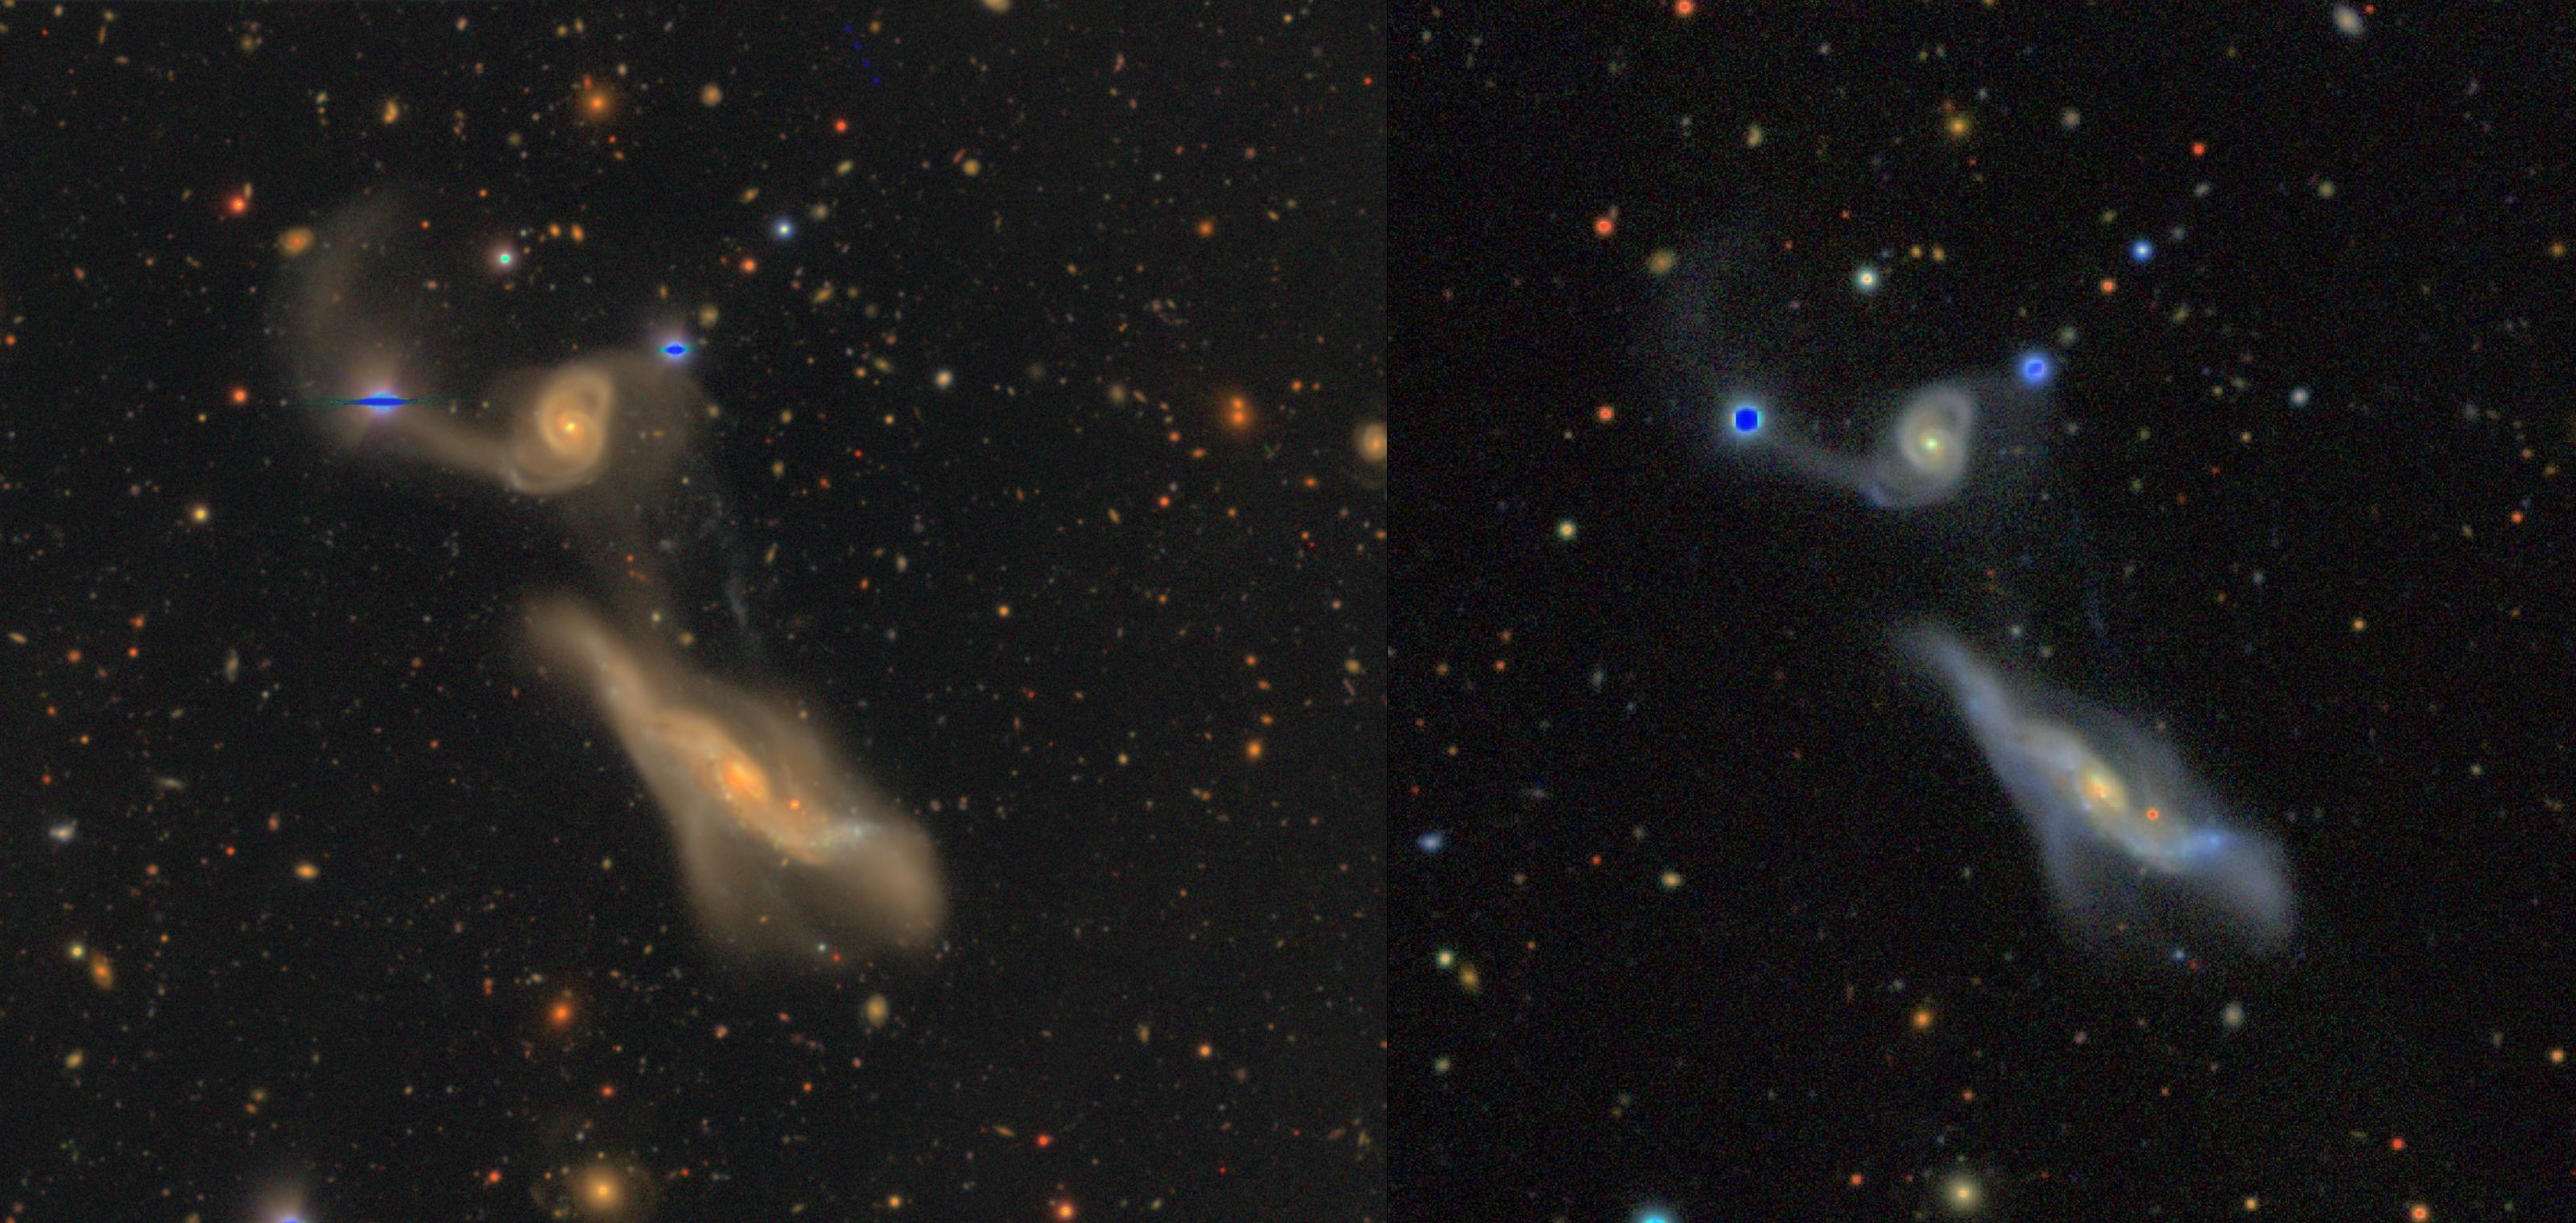
\includegraphics[width=0.9\paperwidth]{HSC-DES-interacting-pair.jpg}} }
        %\colorbox{black}{ \vbox to \paperheight{\vfil\hbox to \paperwidth{\hfil\includegraphics[height=\paperheight]{DES0022-4831-four.jpg}\hfil}\vfil} }
    }
\frame
{
}
}



\frame
{

    \frametitle{Weak Lensing Pipeline Scientist: Research}

    %\setbeamerfont*{itemize/enumerate body}{size=\large}

    \begin{columns}
        \begin{column}{0.5\textwidth}

            \begin{itemize}

                \item Working on an improved deblender based on original
                    MOF from DES.

                \item With a SULI student Lorena Mezini, testing new MOF
                    (see plot) and the Scarlet deblender (Melchior, Moolencamp)
                    for shear measurement.


                  \item The SciDAC postdoc Chi-Ting Chiang (coming Aug
                    2018) will also work on deblending with machine
                    learning methods.

            \end{itemize}
        \end{column}
        \begin{column}{0.5\textwidth}
            \begin{center}
                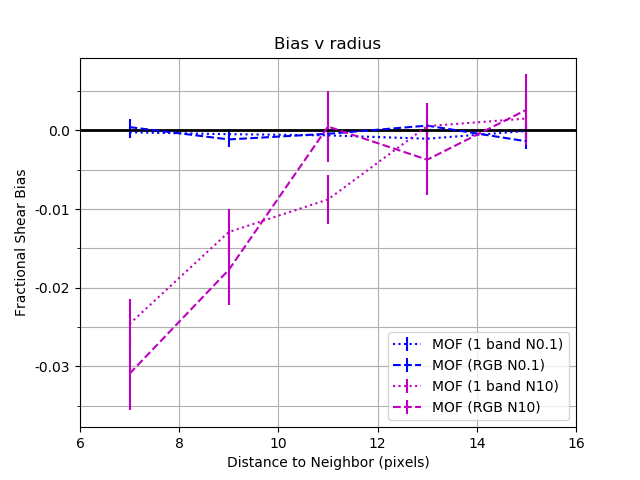
\includegraphics[width=\textwidth]{bias-v-rad-MOF-multiband.png}
            \end{center}
        \end{column}

    \end{columns}

}

\frame
{

    \frametitle{Weak Lensing Pipeline Scientist: Research}

    %\setbeamerfont*{itemize/enumerate body}{size=\large}

    \begin{columns}
        \begin{column}{0.5\textwidth}

            \begin{itemize}

                \item Just finished a project with B. Armstrong showing we can use coadds
                    for shear... if done correctly!
                    
                \item So-called ``postage-stamp
                    coadds''.
                    
                \item Minimal loss of information compared to full multi-epoch
                    approach

                \item Saves LSST a factor of 100 in computing
                    time.
                    
                \item TODO: Write it up and make an implementation
                    available to LSST DM.

            \end{itemize}
        \end{column}
        \begin{column}{0.5\textwidth}
            \begin{center}
                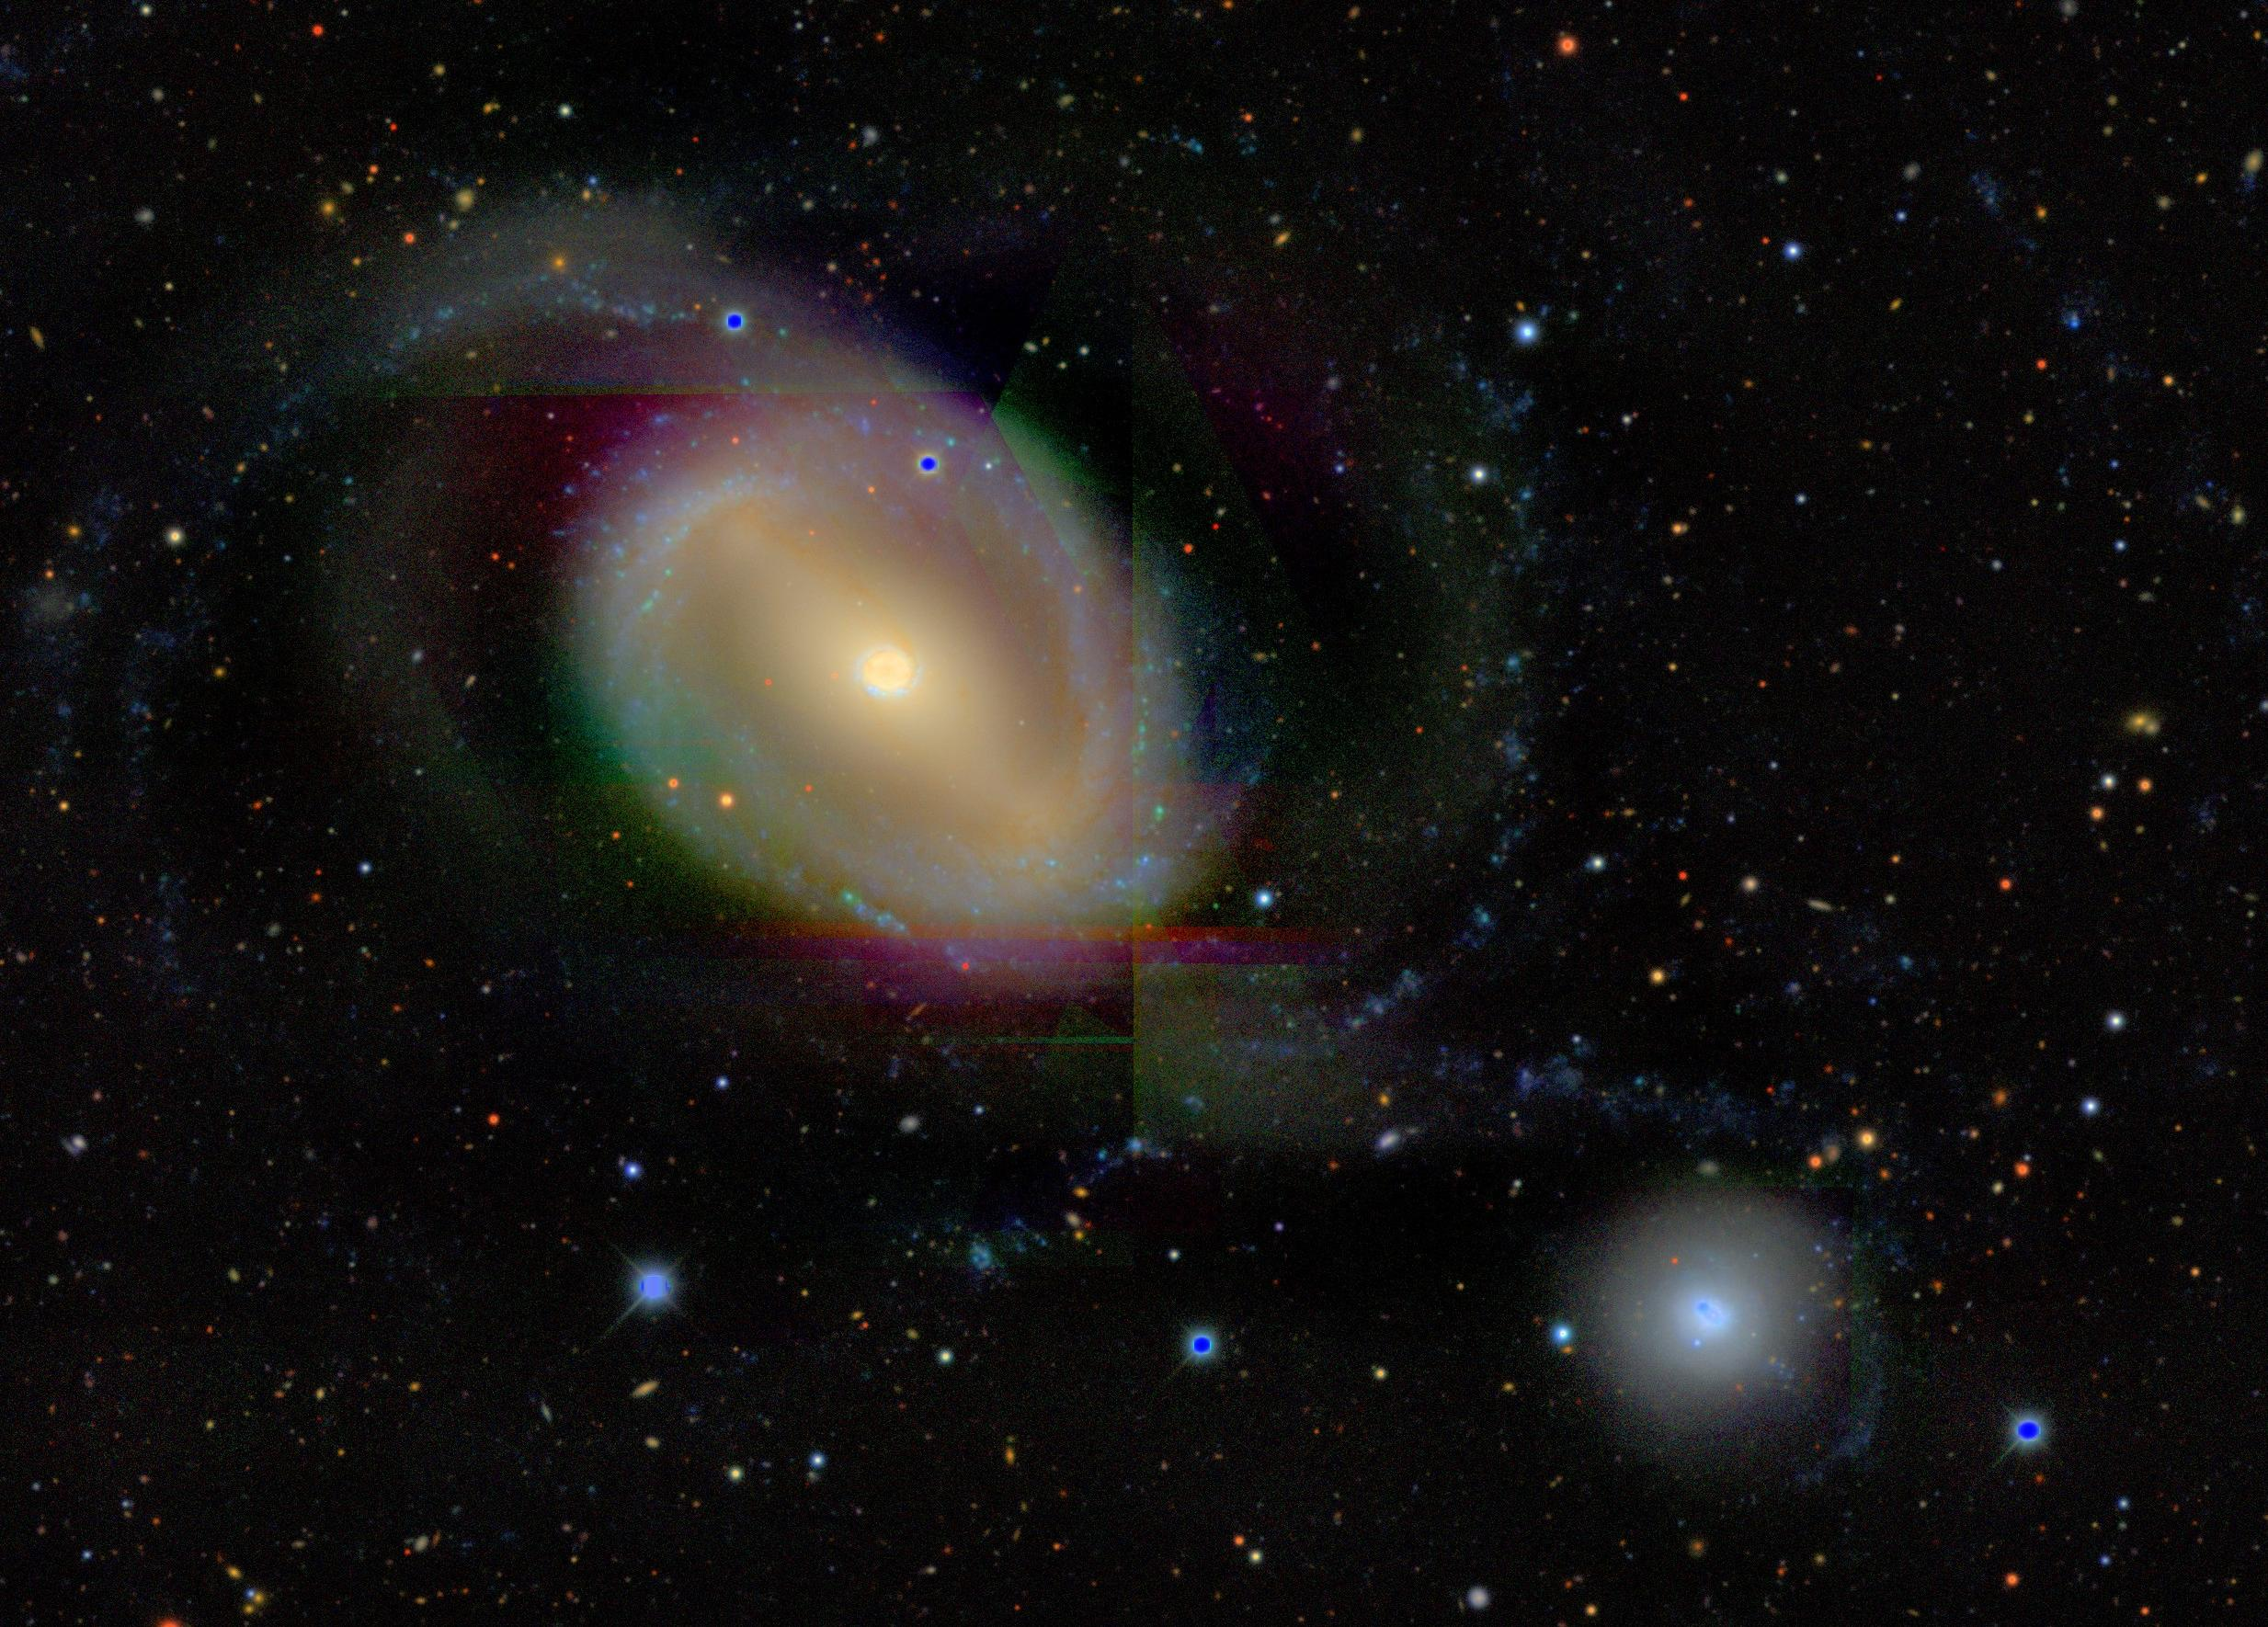
\includegraphics[width=\textwidth,angle=90]{DES0402-4331-discont.jpg}
                \newline
                {\tiny Discontinuities in a coadd }
            \end{center}
        \end{column}

    \end{columns}

}



\frame
{

    \frametitle{Cluster Cosmology with LSST}

    %\setbeamerfont*{itemize/enumerate body}{size=\large}

    \begin{columns}
        \begin{column}{0.5\textwidth}

            \begin{itemize}

                \item Tom McClintock will be joining BNL as a postdoc
                    in Fall 2018.

                \item Tom is the DC2 cluster cosmology project lead.

                \item Leading the the inference of cosmological parameters
                    using cluster lensing.

                \item Tom lead a similar analysis of DES year 1 data, so
                    he is eminently qualified.

            \end{itemize}
        \end{column}

        \begin{column}{0.5\textwidth}
            \begin{center}
                
\includegraphics[width=\textwidth]{TomMportrait.jpg}
                \newline
                {\tiny Tom McClintock}
            \end{center}
        \end{column}

    \end{columns}


}


\frame
{

    \frametitle{Summary}

    %\setbeamerfont*{itemize/enumerate body}{size=\large}

    \begin{columns}
        \begin{column}{0.4\textwidth}
            \begin{itemize}

                \item BNL plays a key role delivering the LSST science rafts

                \item BNL has key leadership and technical roles in the LSST
                    DESC which will expand as current precursor projects
                    wind down (e.g. DES)

                \item BNL is well positioned to have high scientific impact
                    in the LSST era.

            \end{itemize}

        \end{column}
        \begin{column}{0.6\textwidth}
            \centering
                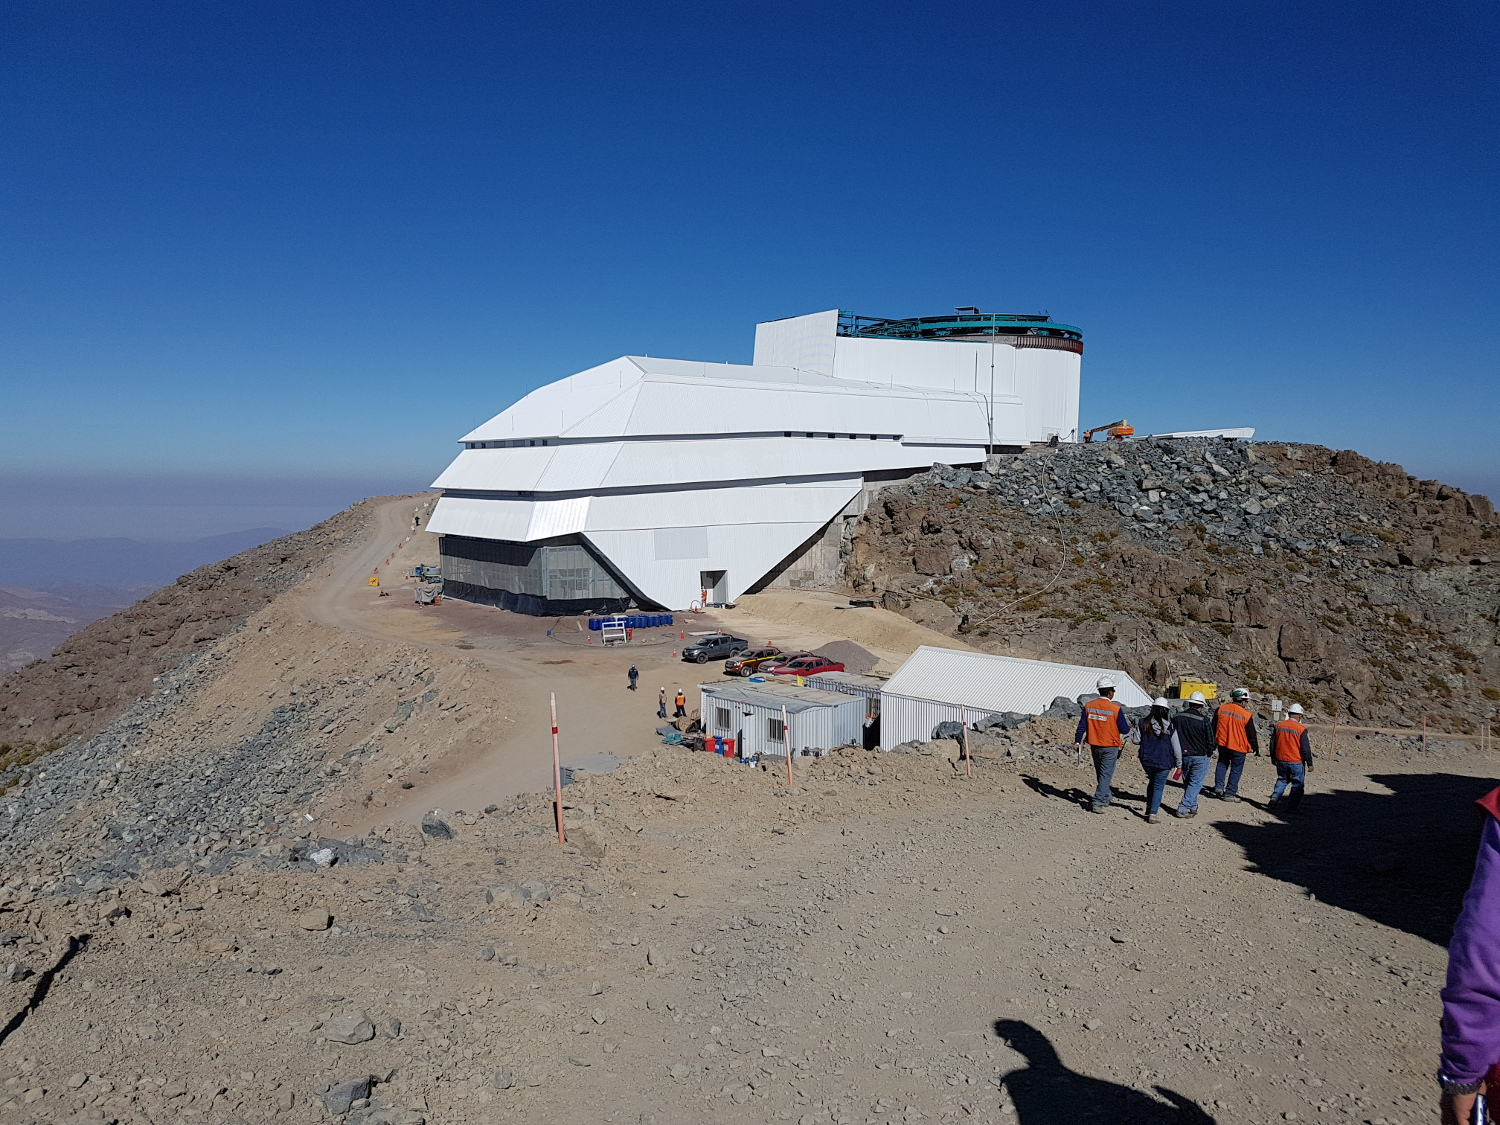
\includegraphics[width=\linewidth]{20180207_101422_scaled.jpg}
                \newline
                {\tiny LSST Project/NSF/AURA}
        \end{column}

    \end{columns}

}






\end{document}
